% ============================================================
% Master's thesis (TFM) -- Master's Degree in Data Science (MDS)
% Facultat d'Informatica de Barcelona (FIB), UPC
%
% Structure follows the "Normativa del treball de fi d'estudis de
% la FIB" (consolidated text, CP.FIB/2024/05/06, 2025/05/08 and
% 2025/10/09):
%   - Art. 12: mandatory cover (fields a-g, plus h for modalities
%     B and D), mandatory abstract, mandatory sustainability and
%     ethics analysis, recommended chapter list.
%   - Art. 61: every document of an MDS thesis is in English.
%   - Art. 62: 30 ECTS x 30 h = 900 h, the budget of docs/roadmap.md.
%   - Art. 65: the sustainability and ethics report is carried out
%     through the gender competence (inclusive language; ethics,
%     equity and bias in data management and analysis).
%
% Planning, methodology and the Gantt chart follow docs/roadmap.md.
% Every \pending{} block says what goes there and which document of
% the repository it is written from; set \showpendingfalse to hide
% them all when compiling a clean draft.
%
% Layout: this file holds the preamble and the order of the parts.
%   frontmatter/   cover, abstract, acknowledgements, acronyms
%   chapters/NN-topic/topic.tex          one folder per chapter
%   chapters/NN-topic/NN-section.tex     a section with no subsections
%   chapters/NN-topic/NN-section/        a section with subsections:
%       section.tex                      its heading and \input list
%       NN-subsection.tex                one file per subsection
%   appendices/    one file per appendix
%   references.bib
% Every \input path is relative to this directory.
%
% Build: latexmk -pdf main.tex   (pdflatex + bibtex)
% ============================================================

\documentclass[11pt,a4paper,oneside]{report}

% ---------- Encoding and language ----------
\usepackage[utf8]{inputenc}
\usepackage[T1]{fontenc}
\usepackage[english]{babel}
\usepackage{lmodern}
\usepackage{microtype}

% ---------- Layout ----------
\usepackage[a4paper,top=2.5cm,bottom=2.5cm,left=3cm,right=2.5cm]{geometry}
\usepackage{setspace}
\onehalfspacing
% Long identifiers in \texttt cannot be hyphenated; let a line stretch
% a little rather than run into the margin.
\setlength{\emergencystretch}{2.5em}
\usepackage{parskip}
\usepackage{pdflscape}
\usepackage{adjustbox}

% ---------- Mathematics ----------
\usepackage{amsmath,amssymb}

% ---------- Tables (booktabs and tabularx are required by
%            sections/custom_dataset.tex and sections/future_work.tex) ----------
\usepackage{booktabs}
\usepackage{tabularx}
\usepackage{longtable}
\usepackage{multirow}
\usepackage{array}

% ---------- Figures ----------
\usepackage{graphicx}
\graphicspath{{figures/}}
\usepackage{float}
\usepackage[font=small,labelfont=bf]{caption}
\usepackage{subcaption}
\usepackage[dvipsnames,table]{xcolor}
\usepackage{tikz}
\usetikzlibrary{positioning,arrows.meta,calc}
\usepackage{pgfgantt}

% ---------- Lists and code ----------
\usepackage{enumitem}
\usepackage{listings}
\lstset{basicstyle=\ttfamily\small, breaklines=true, frame=single,
        columns=fullflexible, keepspaces=true}

% ---------- Bibliography (the section files use \cite) ----------
\usepackage[numbers,sort&compress]{natbib}

% ---------- Links (load last) ----------
\usepackage[hidelinks]{hyperref}
\usepackage{url}

% ---------- Placeholders ----------
\definecolor{pendingcolor}{RGB}{120,120,120}
\newif\ifshowpending
\showpendingtrue          % \showpendingfalse hides every placeholder
\newcommand{\pending}[1]{%
  \ifshowpending
    \par\noindent{\color{pendingcolor}\small\itshape\raggedright\sloppy
    [To write: #1]\par}
  \fi}

% ---------- Gantt styles ----------
\definecolor{ganttdone}{RGB}{120,170,120}
\definecolor{ganttplan}{RGB}{110,150,210}
\definecolor{ganttextra}{RGB}{230,180,90}
\definecolor{ganttpause}{RGB}{200,200,200}

% ============================================================
% Cover data (Art. 12, fields a-h)
% ============================================================
\newcommand{\thesistitle}{[Thesis title]}                         % (a)
\newcommand{\thesisauthor}{Adria Espinoza}                         % (b)
\newcommand{\defencedate}{[Defence date]}                          % (c)
\newcommand{\thesisdirector}{[Director's name]}                    % (d)
\newcommand{\directoraffiliation}{[Department / institution / company]}
% (d) One line per co-director, same format; a ponent (modalities B
% and D) goes on a line below the director(s), same format.
\newcommand{\thesisdegree}{Master's Degree in Data Science}        % (e)
% Official name: Master universitari en Ciencia de Dades (MDS).
% (h) Modalities B and D only: the centre, institution or company
% where the thesis was carried out. Uncomment its line on the cover.
\newcommand{\hostinstitution}{[Company / institution]}

\hypersetup{pdftitle={\thesistitle}, pdfauthor={\thesisauthor}}

% ============================================================

% ============================================================
\begin{document}
% ============================================================

% ---------- Front matter ----------
% ============================================================
% Cover (Art. 12)
% Included from main.tex
% ============================================================

% Cover (Art. 12). The FIB can generate the standard cover; if it
% is used instead, replace this titlepage with
%   \includepdf{cover.pdf}   (\usepackage{pdfpages})
\begin{titlepage}
    \centering
    \IfFileExists{figures/logo-upc-fib.pdf}%
        {\includegraphics[width=0.55\textwidth]{logo-upc-fib.pdf}\par}{}
    \vspace*{2cm}

    {\LARGE\bfseries \thesistitle \par}
    \vspace{2.5cm}

    \begin{tabular}{@{}r@{\hspace{1em}}l@{}}
        \textbf{Author:}        & \thesisauthor \\[0.5em]
        \textbf{Defence date:}  & \defencedate \\[0.5em]
        \textbf{Director:}      & \thesisdirector \\
                                & \textit{\directoraffiliation} \\[0.5em]
        % \textbf{Co-director:} & [Name] \\
        %                       & \textit{[Department / institution / company]} \\[0.5em]
        % \textbf{Ponent:}      & [Name] \\
        %                       & \textit{[Department]} \\[0.5em]
        \textbf{Degree:}        & \thesisdegree \\
        % \textbf{Carried out at:} & \hostinstitution \\  % (h) modalities B and D
    \end{tabular}

    \vfill
    {\large FACULTAT D'INFORMÀTICA DE BARCELONA (FIB)\par}
    \vspace{0.3em}
    {\large UNIVERSITAT POLITÈCNICA DE CATALUNYA (UPC) -- BarcelonaTech\par}
\end{titlepage}


\pagenumbering{roman}
% ============================================================
% Abstract
% Included from main.tex
% ============================================================

\chapter*{Abstract}
\addcontentsline{toc}{chapter}{Abstract}
% Mandatory (Art. 12). MDS requires it in English only (Art. 61);
% the trilingual abstract of Arts. 22, 28, 34 and 39 is for other
% degrees.
\pending{one to two pages: the problem (verifying the claims of
constructive news at a newsroom's pace), the proposed open-web
pipeline, the evaluation (X-Fact and the custom validation set), the
main results with their intervals, and the limitations. Written last.}

\textbf{Keywords:} automated fact-checking, open-domain retrieval,
large language models, constructive journalism, multilingual NLP,
evaluation.

% ============================================================
% Acknowledgements
% Included from main.tex
% ============================================================

\chapter*{Acknowledgements}
\addcontentsline{toc}{chapter}{Acknowledgements}
\pending{optional.}


\tableofcontents
\listoffigures
\listoftables

% ============================================================
% Acronyms
% Included from main.tex
% ============================================================

\chapter*{Acronyms}
\addcontentsline{toc}{chapter}{Acronyms}
\begin{description}[style=nextline,leftmargin=2.5cm,labelwidth=2.2cm]
    \item[API]   Application Programming Interface
    \item[AUC]   Area Under the (ROC) Curve
    \item[ECTS]  European Credit Transfer and Accumulation System
    \item[FIB]   Facultat d'Informàtica de Barcelona
    \item[LLM]   Large Language Model
    \item[MDS]   Master's Degree in Data Science
    \item[NER]   Named Entity Recognition
    \item[NLP]   Natural Language Processing
    \item[RQ]    Research Question
    \item[SDG]   Sustainable Development Goal
    \item[UPC]   Universitat Politècnica de Catalunya
\end{description}


\cleardoublepage
\pagenumbering{arabic}

% ---------- Chapters ----------
% One folder per chapter (chapters/NN-topic/topic.tex). In it, a
% section is one file, or - when it has subsections - a folder
% holding the section file and one file per subsection.
% ============================================================
% Chapter 1: Introduction
% Included from main.tex
% ============================================================

\chapter{Introduction}
\label{ch:introduction}

% ============================================================
% Chapter 1: Introduction
%   Section: Context
% Included from chapters/01-introduction/introduction.tex
% ============================================================

\section{Context}
\label{sec:context}
\pending{misinformation spreads faster than it can be checked by
hand; news distribution optimises for engagement; the news cycle is
dominated by negative content. Source: docs/resumen-ejecutivo.md,
``El problema que resuelve''.}


% ============================================================
% Chapter 1: Introduction
%   Section: Motivation
% Included from chapters/01-introduction/introduction.tex
% ============================================================

\section{Motivation}
\label{sec:motivation}
\pending{why verification has to be part of the flow that produces
and distributes constructive news, not a separate service; why
low-cost and open-web (local models, no paid APIs).}


% ============================================================
% Chapter 1: Introduction
%   Section: Problem Statement
% Included from chapters/01-introduction/introduction.tex
% ============================================================

\section{Problem Statement}
\label{sec:problem}
\pending{the claims of positive-news articles in English and Spanish
mix checkable facts with interpretations of them; no fixed corpus
holds their evidence, so it has to be found on the live web at
verification time.}


% ============================================================
% Chapter 1: Introduction
%   Section: Objectives
% Included from chapters/01-introduction/introduction.tex
% ============================================================

\section{Objectives}
\label{sec:objectives}

% ============================================================
% Chapter 1: Introduction
%   Section: Objectives
%     Subsection: General Objective
% Included from chapters/01-introduction/04-objectives/objectives.tex
% ============================================================

\subsection{General Objective}
\pending{one sentence.}


% ============================================================
% Chapter 1: Introduction
%   Section: Objectives
%     Subsection: Specific Objectives
% Included from chapters/01-introduction/04-objectives/objectives.tex
% ============================================================

\subsection{Specific Objectives}
\pending{one per deliverable of docs/roadmap.md: a discovery and
selection flow for constructive news; an extraction and enrichment
pipeline; an open-web fact-checking pipeline with auditable verdicts;
a labelled validation set and an evaluation harness; a benchmark of
verification and writing models; a reader view.}



% ============================================================
% Chapter 1: Introduction
%   Section: Research Questions
% Included from chapters/01-introduction/introduction.tex
% ============================================================

\section{Research Questions}
\label{sec:research-questions}
% docs/roadmap.md, Phase 4, "Fix 2-3 research questions": whatever
% answers none of them is cut or moved to future work.
\pending{fix the final wording. The roadmap's proposal:}
\begin{description}[leftmargin=1.2cm,labelwidth=1cm]
    \item[RQ1] How well does an open-web, low-cost pipeline verify
    claims from constructive news in Spanish and English, against a
    temporally sound gold set?
    \item[RQ2] Where does it fail: retrieval, ranking or reasoning?
    \item[RQ3] How much of the verification work does it take off a
    journalist?
\end{description}


% ============================================================
% Chapter 1: Introduction
%   Section: Scope
% Included from chapters/01-introduction/introduction.tex
% ============================================================

\section{Scope}
\label{sec:scope}

% ============================================================
% Chapter 1: Introduction
%   Section: Scope
%     Subsection: In Scope
% Included from chapters/01-introduction/06-scope/scope.tex
% ============================================================

\subsection{In Scope}
\pending{discovery and selection, extraction, enrichment,
fact-checking, the graph, the evaluation and the reader view.}


% ============================================================
% Chapter 1: Introduction
%   Section: Scope
%     Subsection: Out of Scope
% Included from chapters/01-introduction/06-scope/scope.tex
% ============================================================

\subsection{Out of Scope}
\pending{cut on 29 September 2026 (docs/roadmap.md, Phase 6): user
accounts, profiles, bookmarks and recommendations; the recommendation
system and the mobile application of docs/arquitectura-tecnica.md
(sections 3 and 4).}



% ============================================================
% Chapter 1: Introduction
%   Section: Structure of the Document
% Included from chapters/01-introduction/introduction.tex
% ============================================================

\section{Structure of the Document}
\label{sec:structure}
\pending{one sentence per chapter.}


% ============================================================
% Chapter 2: State of the Art
% Included from main.tex
% ============================================================

\chapter{State of the Art}
\label{ch:state-of-the-art}

% ============================================================
% Chapter 2: State of the Art
%   Section: Automated Fact-Checking
% Included from chapters/02-state-of-the-art/state-of-the-art.tex
% ============================================================

\section{Automated Fact-Checking}
\label{sec:afc}

% ============================================================
% Chapter 2: State of the Art
%   Section: Automated Fact-Checking
%     Subsection: The Fact-Checking Pipeline
% Included from chapters/02-state-of-the-art/01-automated-fact-checking/automated-fact-checking.tex
% ============================================================

\subsection{The Fact-Checking Pipeline}
\pending{claim detection, evidence retrieval and verdict prediction
\cite{guo2022survey}.}


% ============================================================
% Chapter 2: State of the Art
%   Section: Automated Fact-Checking
%     Subsection: Closed- and Open-Retrieval Verification
% Included from chapters/02-state-of-the-art/01-automated-fact-checking/automated-fact-checking.tex
% ============================================================

\subsection{Closed- and Open-Retrieval Verification}
\pending{FEVER's closed corpus \cite{thorne2018fever} against
real-world, open-web evidence \cite{schlichtkrull2023averitec}; the
leaked-evidence problem \cite{glockner2022missing}. The detailed
argument is in Section~\ref{subsec:discard-justification}; keep only
the overview here.}


% ============================================================
% Chapter 2: State of the Art
%   Section: Automated Fact-Checking
%     Subsection: Language Models as Verifiers
% Included from chapters/02-state-of-the-art/01-automated-fact-checking/automated-fact-checking.tex
% ============================================================

\subsection{Language Models as Verifiers}
\pending{retrieval-augmented verification, citation of evidence,
hallucination and its guardrails.}



% ============================================================
% Chapter 2: State of the Art
%   Section: Benchmarks for Fact Verification
% Included from chapters/02-state-of-the-art/state-of-the-art.tex
% ============================================================

\section{Benchmarks for Fact Verification}
\label{sec:sota-benchmarks}
\pending{FEVER, X-Fact \cite{gupta2021xfact}, AVeriTeC; pointer to
Section~\ref{sec:dataset-selection} for the choice made.}


% ============================================================
% Chapter 2: State of the Art
%   Section: Constructive and Solutions Journalism
% Included from chapters/02-state-of-the-art/state-of-the-art.tex
% ============================================================

\section{Constructive and Solutions Journalism}
\label{sec:constructive-journalism}
\pending{what makes a news item constructive, and why its claims are
harder to check than political statements.}


% ============================================================
% Chapter 2: State of the Art
%   Section: News Discovery, Selection and Recommendation
% Included from chapters/02-state-of-the-art/state-of-the-art.tex
% ============================================================

\section{News Discovery, Selection and Recommendation}
\label{sec:sota-selection}
\pending{news aggregation and editorial selection by people and by
models; graph-based recommendation as the context of
docs/arquitectura-tecnica.md section 3.}


% ============================================================
% Chapter 2: State of the Art
%   Section: Existing Tools and Services
% Included from chapters/02-state-of-the-art/state-of-the-art.tex
% ============================================================

\section{Existing Tools and Services}
\label{sec:sota-tools}
\pending{fact-checking organisations (Newtral and Maldita, rated as
evidence sources and not ingested) and automated tools.}


% ============================================================
% Chapter 2: State of the Art
%   Section: Positioning of This Work
% Included from chapters/02-state-of-the-art/state-of-the-art.tex
% ============================================================

\section{Positioning of This Work}
\label{sec:positioning}
\pending{what no existing system or benchmark covers: open-web
verification of constructive news in English and Spanish, at low
cost, with a verdict that can be audited.}


% ============================================================
% Chapter 3: Project Management
% Included from main.tex
% ============================================================

\chapter{Project Management}
\label{ch:project-management}
% Written from docs/roadmap.md. The roadmap is checked against the
% code, not the plan, and keeps the history of every replanning.

% ============================================================
% Chapter 3: Project Management
%   Section: Methodology
% Included from chapters/03-project-management/project-management.tex
% ============================================================

\section{Methodology}
\label{sec:methodology}

% ============================================================
% Chapter 3: Project Management
%   Section: Methodology
%     Subsection: Iterative Development in Sprints
% Included from chapters/03-project-management/01-methodology/methodology.tex
% ============================================================

\subsection{Iterative Development in Sprints}
\label{subsec:sprints}

The work is organised into phases, and each phase into sprints of one
to three weeks with a budget of hours. Every sprint closes with a
working system: a phase never leaves a stage of the pipeline
half-built for a later one to finish. The first two phases built the
pipeline end to end (Phase~0, foundations) and then stabilised it
(Phase~1); every later phase extends a system that already runs.


% ============================================================
% Chapter 3: Project Management
%   Section: Methodology
%     Subsection: Parallel Tracks
% Included from chapters/03-project-management/01-methodology/methodology.tex
% ============================================================

\subsection{Parallel Tracks}
\label{subsec:tracks}

Since 30 September 2026 the work runs on tracks side by side rather
than one after another:

\begin{itemize}
    \item \textbf{Development} (Phases~2, 3 and~6): scraping,
    fact-checking, the graph, the infrastructure and the interface.
    \item \textbf{Evaluation} (Phase~4): the validation set, the
    harness that runs the pipeline over it, and the tuning those two
    make possible, in that order, since each needs the one before it.
    The model benchmarks (Phase~5) start once Phase~4 has delivered
    labels and a harness to run them on.
    \item \textbf{Testing and quality assurance}, transversal and
    weighted towards the end, because testing follows what each phase
    builds. It ends one week before the report, so that the report
    describes a system that no longer changes.
\end{itemize}


% ============================================================
% Chapter 3: Project Management
%   Section: Methodology
%     Subsection: Definition of Done and Status Tracking
% Included from chapters/03-project-management/01-methodology/methodology.tex
% ============================================================

\subsection{Definition of Done and Status Tracking}
\label{subsec:done}

A task is done when \texttt{./scripts/check.sh} passes: the backend
and inference tests, the frontend typecheck and the labelling tool's
tests. The rules most costly to break are enforced as tests
(\texttt{backend/tests/test\_invariants.py}) rather than kept as
conventions. The roadmap marks each item done, partly done (with
what is left), or not done, and states the verification behind each
mark; it records planned hours, not hours spent.


% ============================================================
% Chapter 3: Project Management
%   Section: Methodology
%     Subsection: Decision Records and Replanning
% Included from chapters/03-project-management/01-methodology/methodology.tex
% ============================================================

\subsection{Decision Records and Replanning}
\label{subsec:replanning}

Every design decision and every incident that motivated one is
written down in \path{docs/decisions/}. The plan is revised when
the evidence changes, keeping the total of 900~hours fixed: a task
that grows is paid for by cutting or shrinking another, and each cut
is recorded with its reason (Section~\ref{sec:deviations}). Work that
answers none of the research questions is cut or moved to future
work.


% ============================================================
% Chapter 3: Project Management
%   Section: Methodology
%     Subsection: Tools
% Included from chapters/03-project-management/01-methodology/methodology.tex
% ============================================================

\subsection{Tools}
\label{subsec:tools}

Git, with a development branch merged into the main one; GitHub
Actions running the same \texttt{check.sh} targets on every push;
Docker Compose for the services; \texttt{uv} and \texttt{npm} for
dependencies.
\pending{follow-up meetings with the director: frequency and format.}



% ============================================================
% Chapter 3: Project Management
%   Section: Planning
% Included from chapters/03-project-management/project-management.tex
% ============================================================

\section{Planning}
\label{sec:planning}

% ============================================================
% Chapter 3: Project Management
%   Section: Planning
%     Subsection: Workload
% Included from chapters/03-project-management/02-planning/planning.tex
% ============================================================

\subsection{Workload}
\label{subsec:workload}

The thesis carries 30~ECTS at 30~hours per credit (Art.~62 of the
FIB regulations), which is the 900~hours the plan distributes. The
weeks run at about 30--35~hours, the pace of Phases~0 and~1, and each
block's dates follow from its hours.


% ============================================================
% Chapter 3: Project Management
%   Section: Planning
%     Subsection: Phases and Tasks
% Included from chapters/03-project-management/02-planning/planning.tex
% ============================================================

\subsection{Phases and Tasks}
\label{subsec:phases}

\begin{table}[H]
\centering
\small
\caption{Phases, dates and planned hours (docs/roadmap.md, rebalanced
on 30 September 2026).}
\label{tab:phases}
\begin{tabularx}{\linewidth}{@{}lXlr@{}}
\toprule
Phase & Content & Dates (2026) & Hours \\
\midrule
0 & Foundations: scraping core, enrichment, fact-checking v1, job
    API and frontend v1 & Jun 1 -- Jul 31 & 300 \\
-- & Vacation pause & Aug 1 -- 31 & 0 \\
1 & Pipeline completion: stabilisation, testing and bugfixing
    & Sep 1 -- 28 & 140 \\
2 & Development: scraping strategies (Sprint 3) and fact-checking
    improvements (Sprint 4) & Sep 29 -- Oct 19 & 120 \\
3 & Neo4j (done on Sep 29) and infrastructure deployment
    & Oct 20 -- Nov 9 & 50 \\
4 & Evaluation: labelling, harness and tuning & Sep 29 -- Nov 16 & 90 \\
5 & AI model testing: writing (Sprint 6) and verification
    (Sprint 7) models & Nov 10 -- Dec 10 & 80 \\
6 & Interface: reader view & Dec 11 -- 17 & 35 \\
-- & Testing and QA, transversal & Sep 29 -- Dec 24 & 50 \\
7 & Thesis report & Dec 25 -- 31 & 35 \\
\midrule
  & \textbf{Total} & & \textbf{900} \\
\bottomrule
\end{tabularx}
\end{table}

\pending{one paragraph per phase with its tasks, taken from the
sprint lists of docs/roadmap.md. The 18 hours of experiments on the
stages before the verdict (added on 5 October) are on top of the 900
and are not yet funded: say where they came from, or report the
overrun.}


% ============================================================
% Chapter 3: Project Management
%   Section: Planning
%     Subsection: Gantt Chart
% Included from chapters/03-project-management/02-planning/planning.tex
% ============================================================

\subsection{Gantt Chart}
\label{subsec:gantt}

Figure~\ref{fig:gantt} shows the plan. Green bars were done when
the plan was last revised; blue bars are planned; the orange bar is
work added on 5 October and not yet funded.

\begin{landscape}
\begin{figure}[p]
\centering
\begin{adjustbox}{max width=\linewidth, max totalheight=0.88\textheight}
\begin{ganttchart}[
    time slot format=isodate,
    x unit=0.075cm,
    y unit title=0.6cm,
    y unit chart=0.48cm,
    hgrid={*1{draw=black!8}},
    title/.append style={fill=black!8, draw=black!30},
    title label font=\footnotesize\bfseries,
    bar label font=\footnotesize,
    group label font=\footnotesize\bfseries,
    milestone label font=\footnotesize\itshape,
    bar/.append style={fill=ganttplan, draw=ganttplan!70!black},
    bar height=0.55,
    group/.append style={fill=black!70},
    group height=0.25,
    group peaks height=0.15,
    group peaks width=2,
    milestone/.append style={fill=BrickRed, draw=BrickRed!70!black},
    milestone height=0.55,
    today=2026-10-06,
    today label={\footnotesize 6 Oct},
    today rule/.style={draw=BrickRed, dashed, thick},
]{2026-06-01}{2026-12-31}
\gantttitlecalendar{month=name} \\
% ---- Phase 0 ----
\ganttgroup{Phase 0: Foundations (300 h)}{2026-06-01}{2026-07-31} \\
\ganttbar[bar/.append style={fill=ganttdone}]{Sprint 0.1: Setup and scraping core (80 h)}{2026-06-01}{2026-06-14} \\
\ganttbar[bar/.append style={fill=ganttdone}]{Sprint 0.2: Enrichment pipeline (80 h)}{2026-06-15}{2026-06-28} \\
\ganttbar[bar/.append style={fill=ganttdone}]{Sprint 0.3: Fact-checking pipeline v1 (80 h)}{2026-06-29}{2026-07-12} \\
\ganttbar[bar/.append style={fill=ganttdone}]{Sprint 0.4: Job API, frontend v1, fixes (60 h)}{2026-07-13}{2026-07-31} \\
\ganttbar[bar/.append style={fill=ganttpause}]{Vacation pause (0 h)}{2026-08-01}{2026-08-31} \\
% ---- Phase 1 ----
\ganttgroup{Phase 1: Pipeline completion (140 h)}{2026-09-01}{2026-09-28} \\
\ganttbar[bar/.append style={fill=ganttdone}]{Sprint 1: Stabilise the core pipeline (70 h)}{2026-09-01}{2026-09-14} \\
\ganttbar[bar/.append style={fill=ganttdone}]{Sprint 2: Testing and bugfixing (70 h)}{2026-09-15}{2026-09-28} \\
% ---- Phase 2 ----
% Sprint 3 was built in September, beside Sprint 2; the roadmap dates
% work already done when it was done and gives it no future calendar.
\ganttgroup{Phase 2: Development (120 h)}{2026-09-15}{2026-10-19} \\
\ganttbar[bar/.append style={fill=ganttdone}]{Sprint 3: Scraping strategies (70 h)}{2026-09-15}{2026-09-28} \\
\ganttbar{Sprint 4: Enrichment and fact-checking (50 h)}{2026-09-29}{2026-10-19} \\
% ---- Phase 3 ----
\ganttgroup{Phase 3: Neo4j and infrastructure (50 h)}{2026-09-29}{2026-11-09} \\
\ganttmilestone{Neo4j integrated (20 h, done)}{2026-09-29} \\
\ganttbar{Infrastructure deployment (30 h)}{2026-10-20}{2026-11-09} \\
% ---- Phase 4 ----
\ganttgroup{Phase 4: Evaluation (90 h)}{2026-09-29}{2026-11-16} \\
\ganttbar{Validation set: label facts 1--150 (34 h)}{2026-09-29}{2026-10-19} \\
\ganttbar{Research questions (3 h)}{2026-10-06}{2026-10-12} \\
\ganttbar{Blind re-label, agreement, join (6 h)}{2026-10-26}{2026-10-30} \\
\ganttmilestone{Labels settled}{2026-10-30} \\
\ganttbar{Evaluation harness (37 h)}{2026-10-20}{2026-11-09} \\
\ganttmilestone{Harness ready}{2026-11-09} \\
\ganttbar[bar/.append style={fill=ganttextra}]{Experiments before the verdict (18 h, unfunded)}{2026-10-06}{2026-11-16} \\
\ganttbar{Tuning against the labels (10 h)}{2026-11-10}{2026-11-16} \\
% ---- Phase 5 ----
\ganttgroup{Phase 5: AI model testing (80 h)}{2026-11-10}{2026-12-10} \\
\ganttbar{Sprint 6: Writing models (20 h)}{2026-11-10}{2026-11-23} \\
\ganttbar{Sprint 7: Verification models (60 h)}{2026-11-17}{2026-12-10} \\
% ---- Phase 6 ----
\ganttgroup{Phase 6: Interface (35 h)}{2026-12-11}{2026-12-17} \\
\ganttbar{Sprint 8: Reader view (35 h)}{2026-12-11}{2026-12-17} \\
% ---- Testing ----
\ganttgroup{Testing and QA, transversal (50 h)}{2026-09-29}{2026-12-24} \\
\ganttbar{October (8 h)}{2026-09-29}{2026-10-31} \\
\ganttbar{November (12 h)}{2026-11-01}{2026-11-30} \\
\ganttbar{December 1--10 (10 h)}{2026-12-01}{2026-12-10} \\
\ganttbar{Final regression and deployment (20 h)}{2026-12-18}{2026-12-24} \\
% ---- Phase 7 ----
\ganttgroup{Phase 7: Thesis report (35 h)}{2026-12-25}{2026-12-31} \\
\ganttbar{Sprint 9: Writing the report (35 h)}{2026-12-25}{2026-12-31}
\end{ganttchart}
\end{adjustbox}
\caption{Gantt chart of the project (docs/roadmap.md, as of
6 October 2026). The dashed line marks the date of this plan.}
\label{fig:gantt}
\end{figure}
\end{landscape}


% ============================================================
% Chapter 3: Project Management
%   Section: Planning
%     Subsection: Milestones
% Included from chapters/03-project-management/02-planning/planning.tex
% ============================================================

\subsection{Milestones}
\label{subsec:milestones}

Besides the project's own milestones (labels settled on 30 October,
harness ready on 9 November), the FIB regulations fix three:

\begin{itemize}
    \item \textbf{Follow-up milestone} (Art.~9): a report on the state
    of the work, presented to the director at about half of it, and
    evaluated positively at least one month before the defence. After
    it, the project's data can no longer be changed, and
    confidentiality can no longer be requested (Art.~15).
    \item \textbf{Final report accepted} by the director at least
    seven days before the defence (Art.~10).
    \item \textbf{Defence} in public before a panel of three members
    of the FIB teaching staff (Art.~11).
\end{itemize}
\pending{the dates of the follow-up milestone, the delivery and the
defence, once the defence period is chosen.}



% ============================================================
% Chapter 3: Project Management
%   Section: Deviations from the Initial Plan
% Included from chapters/03-project-management/project-management.tex
% ============================================================

\section{Deviations from the Initial Plan}
\label{sec:deviations}

The plan was rebalanced three times, always at 900 hours
(Table~\ref{tab:rebalance}).

\begin{table}[H]
\centering
\small
\caption{Hours per phase after each replanning (docs/roadmap.md). The
earlier columns are regrouped into the current phases so that the
three add up the same way.}
\label{tab:rebalance}
\begin{tabular}{@{}lrrr@{}}
\toprule
Phase & Sep 28 & Sep 29 & Sep 30 \\
\midrule
0: Foundations                      & 300 & 300 & 300 \\
1: Pipeline completion              & 140 & 140 & 140 \\
2: Development                      & 140 & 130 & 120 \\
3: Neo4j and infrastructure         &  70 &  65 &  50 \\
4: Evaluation                       &  40 &  80 &  90 \\
5: AI model testing                 & 120 &  80 &  80 \\
6: Interface                        &  40 &  20 &  35 \\
Testing and QA, transversal         &   0 &  50 &  50 \\
7: Thesis report                    &  50 &  35 &  35 \\
\midrule
\textbf{Total}                      & \textbf{900} & \textbf{900} & \textbf{900} \\
\bottomrule
\end{tabular}
\end{table}

\pending{the reason for each change, from the roadmap's header:
the validation set turned out to be a 40-hour task (Sep 28); its own
window, a testing track, the evaluation harness and the search fix,
paid for by cutting the user-facing application to a reader view and
two hosted-model benchmarks (Sep 29); dates derived from hours, two
parallel tracks, Neo4j done in less than planned (Sep 30); the 18
unfunded hours of experiments (Oct 5). Close with the deviations
found after this plan.}


% ============================================================
% Chapter 3: Project Management
%   Section: Risk Management
% Included from chapters/03-project-management/project-management.tex
% ============================================================

\section{Risk Management}
\label{sec:risks}
\pending{one row per risk with its probability, impact and
mitigation, each one observed during the project
(docs/roadmap.md, CLAUDE.md ``Known slow / known unverified''):
search engines refusing automated queries (68 of 69 empty on
25 September; \texttt{searchUnavailable} and the fallback route);
the LLM timing out on a CPU (3 of 4 verdicts on 1 October; separate
production limits); sources blocking the scraper (EFE and Reuters
disabled on 6 October); the labelling taking longer than planned
(rebalance of 28 September); the cloud deployment never applied to a
real project.}


% ============================================================
% Chapter 3: Project Management
%   Section: Budget
% Included from chapters/03-project-management/project-management.tex
% ============================================================

\section{Budget}
\label{sec:budget}

% ============================================================
% Chapter 3: Project Management
%   Section: Budget
%     Subsection: Personnel Costs
% Included from chapters/03-project-management/05-budget/budget.tex
% ============================================================

\subsection{Personnel Costs}
\pending{hours per role (project manager, developer, data scientist,
tester) from Table~\ref{tab:phases}, times an hourly rate with its
source.}


% ============================================================
% Chapter 3: Project Management
%   Section: Budget
%     Subsection: Hardware and Software Costs
% Included from chapters/03-project-management/05-budget/budget.tex
% ============================================================

\subsection{Hardware and Software Costs}
\pending{the development laptop (GPU) amortised over the project;
every software component is open source.}


% ============================================================
% Chapter 3: Project Management
%   Section: Budget
%     Subsection: Infrastructure Costs
% Included from chapters/03-project-management/05-budget/budget.tex
% ============================================================

\subsection{Infrastructure Costs}
\pending{one e2-standard-4 Compute Engine VM in Madrid, about 115~USD
a month on demand (docs/decisions/deployment.md); hosted LLM
providers priced per run in backend/data/evaluation/prices.json.}


% ============================================================
% Chapter 3: Project Management
%   Section: Budget
%     Subsection: Contingency and Total
% Included from chapters/03-project-management/05-budget/budget.tex
% ============================================================

\subsection{Contingency and Total}
\pending{contingency margin, unforeseen costs and the total.}



% ============================================================
% Chapter 4: Proposed Method: Specification and Design
% Included from main.tex
% ============================================================

\chapter{Proposed Method: Specification and Design}
\label{ch:methodology}
% Label kept as ch:methodology: sections/evaluation_dataset.tex
% refers here as the chapter that describes the system.

% ============================================================
% Chapter 4: Proposed Method: Specification and Design
%   Section: Requirements
% Included from chapters/04-proposed-method/proposed-method.tex
% ============================================================

\section{Requirements}
\label{sec:requirements}

% ============================================================
% Chapter 4: Proposed Method: Specification and Design
%   Section: Requirements
%     Subsection: Functional Requirements
% Included from chapters/04-proposed-method/01-requirements/requirements.tex
% ============================================================

\subsection{Functional Requirements}
\pending{discover, select, extract, enrich, admit, verify, store,
publish; per-claim verdicts with cited evidence.}


% ============================================================
% Chapter 4: Proposed Method: Specification and Design
%   Section: Requirements
%     Subsection: Non-Functional Requirements
% Included from chapters/04-proposed-method/01-requirements/requirements.tex
% ============================================================

\subsection{Non-Functional Requirements}
\pending{low cost (local models, no paid APIs), auditability (every
step journalled), fail towards caution, English and Spanish,
reproducible evaluation.}



% ============================================================
% Chapter 4: Proposed Method: Specification and Design
%   Section: System Architecture
% Included from chapters/04-proposed-method/proposed-method.tex
% ============================================================

\section{System Architecture}
\label{sec:architecture}
\pending{the services and how they talk: backend, inference
service, frontend, SearXNG, Qdrant, Neo4j, Ollama. Source:
docs/arquitectura-tecnica.md section 2.1 (topology diagram) and
docs/decisions/inference.md.}


% ============================================================
% Chapter 4: Proposed Method: Specification and Design
%   Section: Data Architecture
% Included from chapters/04-proposed-method/proposed-method.tex
% ============================================================

\section{Data Architecture}
\label{sec:data-architecture}
\pending{the three-layer lake (raw, processed, exploitation) with
lineage, the vector store and the graph schema. Sources:
docs/decisions/storage.md, docs/decisions/graph.md.}


% ============================================================
% Chapter 4: Proposed Method: Specification and Design
%   Section: Candidate Selection
% Included from chapters/04-proposed-method/proposed-method.tex
% ============================================================

\section{Candidate Selection}
\label{sec:design-selection}
\pending{what happens between discovery and analysis: the mission
screen, candidate ranking and the choice of up to twenty by a person
or the AI. How the candidates are found is
Section~\ref{sec:dev-scraping}. Source: docs/decisions/selection.md.}


% ============================================================
% Chapter 4: Proposed Method: Specification and Design
%   Section: Enrichment
% Included from chapters/04-proposed-method/proposed-method.tex
% ============================================================

\section{Enrichment}
\label{sec:design-enrichment}
\pending{keywords, entities, claims, topic, sentiment and embeddings,
computed over the text the extraction cascade
(Section~\ref{subsec:scraping-cascade}) returns. Source:
docs/arquitectura-tecnica.md section 2.3.}


% ============================================================
% Chapter 4: Proposed Method: Specification and Design
%   Section: The Fact-Checking Pipeline
% Included from chapters/04-proposed-method/proposed-method.tex
% ============================================================

\section{The Fact-Checking Pipeline}
\label{sec:design-fact-checking}
\pending{reconcile with the six stages listed in
sections/evaluation\_dataset.tex: docs/arquitectura-tecnica.md
section 2.4 describes seven.}

% ============================================================
% Chapter 4: Proposed Method: Specification and Design
%   Section: The Fact-Checking Pipeline
%     Subsection: Admission Filter
% Included from chapters/04-proposed-method/06-fact-checking-pipeline/fact-checking-pipeline.tex
% ============================================================

\subsection{Admission Filter}
\pending{docs/arquitectura-tecnica.md 2.4.1;
backend/src/services/admission/README.md.}


% ============================================================
% Chapter 4: Proposed Method: Specification and Design
%   Section: The Fact-Checking Pipeline
%     Subsection: Claim Selection
% Included from chapters/04-proposed-method/06-fact-checking-pipeline/fact-checking-pipeline.tex
% ============================================================

\subsection{Claim Selection}
\pending{anchor claims, ranked by how load-bearing they are.}


% ============================================================
% Chapter 4: Proposed Method: Specification and Design
%   Section: The Fact-Checking Pipeline
%     Subsection: Evidence Retrieval
% Included from chapters/04-proposed-method/06-fact-checking-pipeline/fact-checking-pipeline.tex
% ============================================================

\subsection{Evidence Retrieval}
\pending{three queries per claim fused by reciprocal rank; search
unavailable as its own state. Source: docs/decisions/retrieval.md.}


% ============================================================
% Chapter 4: Proposed Method: Specification and Design
%   Section: The Fact-Checking Pipeline
%     Subsection: Evidence Ranking and the Pertinence Gate
% Included from chapters/04-proposed-method/06-fact-checking-pipeline/fact-checking-pipeline.tex
% ============================================================

\subsection{Evidence Ranking and the Pertinence Gate}
\pending{similarity, recency, reliability and term coverage; the
gate that cuts off-target sources before the model sees them.}


% ============================================================
% Chapter 4: Proposed Method: Specification and Design
%   Section: The Fact-Checking Pipeline
%     Subsection: Verification with a Language Model
% Included from chapters/04-proposed-method/06-fact-checking-pipeline/fact-checking-pipeline.tex
% ============================================================

\subsection{Verification with a Language Model}
\pending{a closed classification forced to cite its sources.}


% ============================================================
% Chapter 4: Proposed Method: Specification and Design
%   Section: The Fact-Checking Pipeline
%     Subsection: Confidence Recalibration
% Included from chapters/04-proposed-method/06-fact-checking-pipeline/fact-checking-pipeline.tex
% ============================================================

\subsection{Confidence Recalibration}
\pending{confidence that does not depend on the model's own
introspection; the hard UNVERIFIED fallback.}


% ============================================================
% Chapter 4: Proposed Method: Specification and Design
%   Section: The Fact-Checking Pipeline
%     Subsection: Article-Level Aggregation
% Included from chapters/04-proposed-method/06-fact-checking-pipeline/fact-checking-pipeline.tex
% ============================================================

\subsection{Article-Level Aggregation}
\pending{worst-claim-wins and its known limitation.}



% ============================================================
% Chapter 4: Proposed Method: Specification and Design
%   Section: Concurrency Design
% Included from chapters/04-proposed-method/proposed-method.tex
% ============================================================

\section{Concurrency Design}
\label{sec:design-concurrency}
\pending{claims checked concurrently, each claim's stages
sequential; resource ceilings per external service; results in input
order. Source: docs/decisions/concurrency.md.}


% ============================================================
% Chapter 4: Proposed Method: Specification and Design
%   Section: Interface Design
% Included from chapters/04-proposed-method/proposed-method.tex
% ============================================================

\section{Interface Design}
\label{sec:design-interface}
\pending{the newsroom flow (Discover, Analyze, Live, Reader), the
lab tools and the public reader view. Source: frontend/CLAUDE.md.}


% ============================================================
% Chapter 5: Development
% Included from main.tex
% ============================================================

\chapter{Development}
\label{ch:development}

% ============================================================
% Chapter 5: Development
%   Section: Technology Stack
% Included from chapters/05-development/development.tex
% ============================================================

\section{Technology Stack}
\label{sec:stack}
\pending{Python and FastAPI, Next.js and TypeScript, Docker Compose;
the models (GLiNER, the sentiment classifier, bge-m3, the LLM via
Ollama) and why each was chosen.}


% ============================================================
% Chapter 5: Development
%   Section: News Acquisition: Discovery and Extraction
% Included from chapters/05-development/development.tex
%
% Written from docs/decisions/scraping.md, docs/decisions/selection.md
% (discovery), backend/data/sources/README.md, the code under
% backend/src/services/scraper/ and the dated measurements in
% docs/roadmap.md.
% ============================================================

\section{News Acquisition: Discovery and Extraction}
\label{sec:dev-scraping}

Every article the system analyses, and every web page it reads as
evidence, is obtained by the acquisition layer described in this
section. Its job is narrow and adversarial at the same time: find the
articles a configured news source has published recently, and turn any
URL into clean article text with its title, author and publication
time, while the servers on the other side are slow, inconsistent,
occasionally hostile to automated clients, and never under the
system's control. The layer is implemented in
\path{backend/src/services/scraper/} and is shared by every part of the
pipeline that needs a page.

% ============================================================
% Chapter 5: Development
%   Section: News Acquisition: Discovery and Extraction
%     Subsection: Overview
% Included from chapters/05-development/02-news-acquisition/news-acquisition.tex
% ============================================================

\subsection{Overview}
\label{subsec:scraping-overview}

Acquisition is two steps, composed by the \texttt{Scraper} class
(Figure~\ref{fig:acquisition}):

\begin{enumerate}
    \item \textbf{Discovery} (\texttt{DiscoveryService}) takes a
    configured source and returns the URLs of its recent articles,
    together with whatever the source says about each one before it is
    opened: a title, a summary and a publication time.
    \item \textbf{Extraction} (\texttt{ExtractorService}) takes one
    URL and returns the article: its body, title, author, date and,
    when the page states it, the publication time to the minute.
\end{enumerate}

The two steps are used separately. Discovery feeds the candidate
rounds from which a person or the AI chooses what to analyse
(Section~\ref{sec:design-selection}), the one-shot ingestion endpoint
and the daily labelling batch. Extraction is called for every chosen
candidate, for every URL posted to the analysis endpoint, for every
web page read as evidence for a claim, and by the tools that check the
sources' health. Each call states its \emph{purpose}
(\texttt{article}, \texttt{evidence}, \texttt{enrichment},
\texttt{ingestion}, \texttt{discovery}, \texttt{source\_check},
\texttt{probe}, \texttt{labelling}), which decides how much the call
may spend and under which heading it is counted.

Four principles run through the implementation, each introduced after
a measured failure that is cited where it is described:

\begin{itemize}
    \item \textbf{Cheapest first.} Discovery and extraction both try
    their strategies in order of cost, and only go to the next one when
    it could plausibly succeed where the previous one failed.
    \item \textbf{Every fetch is guarded.} Every URL is checked against
    an address-based guard before any request is sent, and again at
    every redirect.
    \item \textbf{Everything is counted.} Every page wanted is recorded
    with its outcome, the strategies tried and the requests actually
    sent, so a source that stops working shows up as such rather than
    as an absence of news.
    \item \textbf{Sources are configuration, not code.} Adding a source
    means adding a YAML file; nothing in the code names a particular
    outlet.
\end{itemize}

\begin{figure}[ht]
\centering
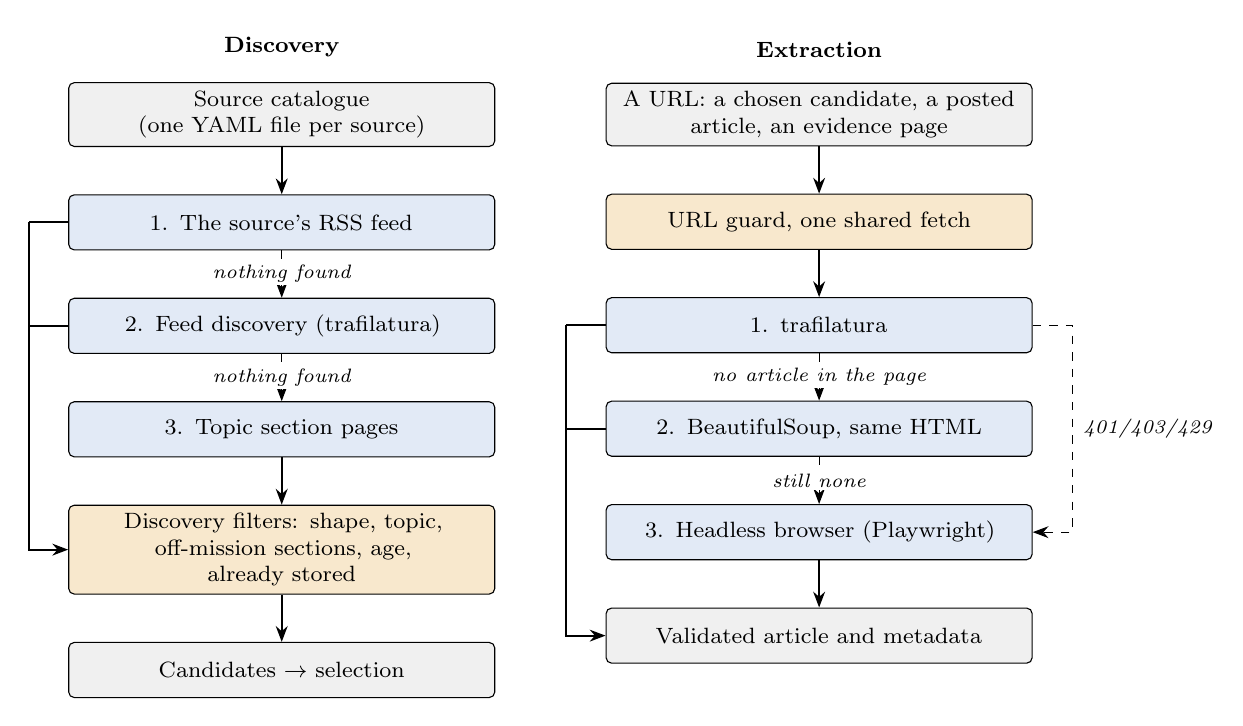
\begin{tikzpicture}[
    node distance=6mm and 14mm,
    box/.style={draw, rounded corners=2pt, align=center,
                font=\footnotesize, text width=5.2cm,
                minimum height=7mm, inner sep=3pt},
    io/.style={box, fill=black!6},
    stage/.style={box, fill=ganttplan!20},
    gate/.style={box, fill=ganttextra!30},
    arr/.style={-{Stealth[length=2mm]}, thick},
    alt/.style={-{Stealth[length=2mm]}, dashed},
    lbl/.style={font=\scriptsize\itshape, fill=white, inner sep=1pt},
]
% ---- Discovery ----
\node[io]                   (src)    {Source catalogue\\(one YAML file per source)};
\node[stage, below=of src]  (rss)    {1. The source's RSS feed};
\node[stage, below=of rss]  (feeds)  {2. Feed discovery (trafilatura)};
\node[stage, below=of feeds](pages)  {3. Topic section pages};
\node[gate,  below=of pages](filt)   {Discovery filters: shape, topic,\\
                                      off-mission sections, age,\\
                                      already stored};
\node[io,    below=of filt] (round)  {Candidates $\rightarrow$ selection};

\draw[arr] (src) -- (rss);
\draw[alt] (rss) -- node[lbl]{nothing found} (feeds);
\draw[alt] (feeds) -- node[lbl]{nothing found} (pages);
\draw[arr] (pages) -- (filt);
\draw[arr] (filt) -- (round);
\coordinate (dl) at ($(rss.west)+(-5mm,0)$);
\draw[thick] (rss.west) -- (dl);
\draw[thick] (feeds.west) -- (dl |- feeds.west);
\draw[arr] (dl) |- (filt.west);

% ---- Extraction ----
\node[io,    right=of src]  (in)     {A URL: a chosen candidate, a posted\\article, an evidence page};
\node[gate,  below=of in]   (guard)  {URL guard, one shared fetch};
\node[stage, below=of guard](traf)   {1. trafilatura};
\node[stage, below=of traf] (bs)     {2. BeautifulSoup, same HTML};
\node[stage, below=of bs]   (pw)     {3. Headless browser (Playwright)};
\node[io,    below=of pw]   (out)    {Validated article and metadata};

\draw[arr] (in) -- (guard);
\draw[arr] (guard) -- (traf);
\draw[alt] (traf) -- node[lbl]{no article in the page} (bs);
\draw[alt] (bs) -- node[lbl]{still none} (pw);
\draw[alt] (traf.east) -- ++(5mm,0) |- node[lbl, pos=0.25, right, xshift=1mm]{401/403/429} (pw.east);
\draw[arr] (pw) -- (out);
\coordinate (el) at ($(traf.west)+(-5mm,0)$);
\draw[thick] (traf.west) -- (el);
\draw[thick] (bs.west) -- (el |- bs.west);
\draw[arr] (el) |- (out.west);

\node[font=\footnotesize\bfseries, above=2mm of src] {Discovery};
\node[font=\footnotesize\bfseries, above=2mm of in]  {Extraction};
\end{tikzpicture}
\caption{The acquisition layer. Solid arrows are the normal path;
dashed arrows are escalations, taken only when the previous step could
not help. A missing page, a timeout or a guard refusal stops the
extraction at once.}
\label{fig:acquisition}
\end{figure}


% ============================================================
% Chapter 5: Development
%   Section: News Acquisition: Discovery and Extraction
%     Subsection: The Source Catalogue
% Included from chapters/05-development/02-news-acquisition/news-acquisition.tex
% ============================================================

\subsection{The Source Catalogue}
\label{subsec:scraping-sources}

Each news source is one YAML file in \path{backend/data/sources/},
loaded by \texttt{SourceRepository} into a \texttt{NewsSource} model.
Only an identifier, a name and a base URL are required; the fields
that matter to acquisition are listed in
Table~\ref{tab:source-fields}.

\begin{table}[ht]
\centering
\small
\caption{Fields of a source that acquisition reads.}
\label{tab:source-fields}
\begin{tabularx}{\linewidth}{@{}lX@{}}
\toprule
Field & Use \\
\midrule
\texttt{rss\_url}             & The feed read first by discovery. \\
\texttt{language}             & \texttt{en} or \texttt{es}; selects the
                                 keyword lists and section names used to
                                 filter its links. \\
\texttt{groups}               & The topic groups the source has real
                                 sections for
                                 (Section~\ref{subsec:scraping-groups}). \\
\texttt{reliability\_index}   & Editorial reliability in $[0,1]$, used
                                 when its pages are ranked as evidence
                                 and when its candidates are ranked. \\
\texttt{enabled}              & Whether the source is ingested at all. \\
\texttt{requires\_javascript} & Sends its articles to the browser first
                                 (Section~\ref{subsec:scraping-cascade}). \\
\texttt{positive\_editorial}  & The outlet publishes only positive news;
                                 the mission screen does not apply to it. \\
\texttt{metadata.selectors}   & Optional CSS selectors for the title,
                                 body, author and date, for layouts no
                                 generic parser understands. \\
\bottomrule
\end{tabularx}
\end{table}

\paragraph{Composition.} The catalogue holds 36 sources, 20 in English
and 16 in Spanish: 26 news outlets, four public bodies (NASA, the
European Space Agency, the World Health Organization and UN News), four
academic publishers (MIT News, \textit{Nature}, The Conversation and
Yale Environment 360) and two blogs. Three of them (Good News Network,
Positive News and Reasons to be Cheerful) publish only positive news.
Appendix~\ref{app:sources} lists them all.

\paragraph{Enabled and disabled.} 32 sources are enabled, 19 in English
and 13 in Spanish. A disabled source is not ingested, probed or
recognised from a posted URL, but it is still read by the reliability
map, so its pages keep their rating when they are found as evidence.
That is the mechanism for rating a domain without ingesting it, and it
is used for two different reasons. The fact-checkers Newtral and
Maldita are disabled because a fact-check quotes the claim it
debunks, and claim extraction would take that quotation for the
article's own claim. Agencia EFE and Reuters are disabled because they
refused every request from 23~September to 6~October~2026 (HTTP 403
and 401 respectively).

\paragraph{One source per domain.} Reliability and the recognition of
posted URLs are both looked up by domain, so a second file on the same
domain (BBC Mundo on \texttt{bbc.com}, for instance) would silently
override the first. A test of the repository fails on any such pair.

\paragraph{How a source is admitted.} The catalogue grew from 12 to 36
sources on 28~September~2026, and every addition passed the same test
before its file was committed: its feed had to produce article links,
and two of those articles had to extract through the real cascade.
Seven candidates failed it: NPR, Phys.org and El Confidencial (the
feed worked, the articles would not extract), ScienceDaily, DW Español
and CSIC (no article links in the feed) and the Associated Press
(HTTP 403). RTVE's dead feed was replaced the same day.


% ============================================================
% Chapter 5: Development
%   Section: News Acquisition: Discovery and Extraction
%     Subsection: The Shared Fetcher and the URL Guard
% Included from chapters/05-development/02-news-acquisition/news-acquisition.tex
% ============================================================

\subsection{The Shared Fetcher and the URL Guard}
\label{subsec:scraping-fetcher}

\paragraph{One fetch per page.} Every HTTP request of the acquisition
layer goes through one class, \texttt{Fetcher}
(\path{services/scraper/fetcher.py}). It sends a single \texttt{GET}
with a 20-second timeout and a User-Agent that names the system
(\texttt{InspiringNewsBot/1.0}), and returns the page as the server
sent it. The HTML parsers of the extraction cascade share that page:
before this, each strategy fetched for itself, so falling back to a
second parser doubled the requests sent to exactly the sites that were
already the hardest to scrape. Only a strategy that needs something
plain HTML cannot give, a rendered page, goes back to the network.

\paragraph{The URL guard.} All fetching happens on the server, and the
URLs come from outside: the analysis endpoint takes them from its
caller, and evidence retrieval from whatever the search engine
returned. Without a check, the service would be an HTTP proxy into its
own network. In the development stack that network contains the graph
database and the search engine, and on a cloud host the instance
metadata endpoint is one request away. The guard
(\path{services/scraper/url_guard.py}) is therefore applied to every
URL before it is fetched, and it is deny-by-address rather than
allow-by-domain: an allow-list of news domains would defeat the purpose
of an endpoint that accepts any article the user found, while what must
never be reachable is the infrastructure, which is a question of
address space. A URL is refused when:

\begin{itemize}
    \item its scheme is not \texttt{http} or \texttt{https}, or it has
    no host;
    \item its port is one of twelve ports used by internal services and
    never by a public web page (SSH, SMTP, SMB, PostgreSQL, MySQL,
    Redis, Neo4j's two ports, Elasticsearch, Memcached, MongoDB and
    Telnet);
    \item any address its host resolves to is private, loopback,
    link-local (where cloud metadata services live), reserved,
    multicast or unspecified. The name is resolved by the guard itself
    rather than trusted, because a public name can have the address
    \texttt{127.0.0.1}, and a name that resolves to both a public and a
    private address is refused.
\end{itemize}

A host that does not resolve at all is still refused, but counted as a
connection failure rather than as a block, since a mistyped or dead
domain is not the guard protecting anything. An explicit list of
allowed hosts, empty by default, exists for staging servers on a
private network, so that nobody has to switch the guard off to reach
one.

\paragraph{Redirects.} An HTTP library that follows redirects by
itself would walk straight past the guard: a public URL can redirect
to \texttt{127.0.0.1}. The fetcher therefore follows redirects itself,
one hop at a time, checking each new location with the guard, and
gives up after five.

\paragraph{Outcomes.} A failed fetch is classified once, in the same
way for discovery and for extraction, so that a 403 on a feed and a
403 on an article are counted alike. Table~\ref{tab:fetch-outcomes}
lists the outcomes; only \texttt{ok} produced an article.

\begin{table}[ht]
\centering
\small
\caption{Outcomes of an extraction attempt.}
\label{tab:fetch-outcomes}
\begin{tabularx}{\linewidth}{@{}lX@{}}
\toprule
Outcome & Meaning \\
\midrule
\texttt{ok}                & An article was extracted. \\
\texttt{too\_short}        & Parsed, but shorter than the run's minimum
                             body length: a paywall stub, a cookie wall,
                             a gallery. \\
\texttt{no\_content}       & Fetched, but no article text was found. \\
\texttt{http\_error}       & The server answered 4xx or 5xx (the status
                             is kept). \\
\texttt{timeout}, \texttt{connection\_error} & The server did not
                             answer, or could not be reached. \\
\texttt{blocked}           & Refused by the URL guard; never sent. \\
\texttt{unavailable}       & The strategy cannot run here (no headless
                             browser installed). \\
\texttt{error}             & Anything else. \\
\bottomrule
\end{tabularx}
\end{table}


% ============================================================
% Chapter 5: Development
%   Section: News Acquisition: Discovery and Extraction
%     Subsection: Discovery Strategies
% Included from chapters/05-development/02-news-acquisition/news-acquisition.tex
% ============================================================

\subsection{Discovery Strategies}
\label{subsec:scraping-discovery}

Discovery tries three strategies per source, cheapest first, and stops
at the first that returns links (Table~\ref{tab:discovery-strategies}).
Every attempt is recorded under the purpose \texttt{discovery}, so a
feed that starts failing appears on the monitoring page next to the
articles it no longer delivers.

\begin{table}[ht]
\centering
\small
\caption{Discovery strategies, in the order they are tried.}
\label{tab:discovery-strategies}
\begin{tabularx}{\linewidth}{@{}lXl@{}}
\toprule
Strategy & Tried when & Gives per link \\
\midrule
1. RSS feed            & Always, if the source has a feed URL.
                       & time, title, summary \\
2. Feed discovery      & The feed gave nothing: it is searched for on
                         the feed URL and then on the homepage.
                       & URL only \\
3. Topic section pages & There is no feed at all.
                       & URL only \\
\bottomrule
\end{tabularx}
\end{table}

\paragraph{The RSS feed.} The feed is downloaded through the shared
fetcher, so it is guarded and has a timeout (the feed library's own
HTTP client has neither), and is then parsed with \texttt{feedparser}.
Each item keeps its publication time (in UTC), its title and a summary
reduced to 400 characters of plain text: what the candidate list shows
and the AI selection reads before any article is opened. On
4~October~2026, all 1,248 URLs from the 29 feeds that answered carried
a time.

\paragraph{Feed discovery.} When the configured feed yields nothing,
\texttt{trafilatura}'s feed discovery looks for one, first on the
configured feed URL and then on the homepage. It is lenient with
malformed XML and finds the feed a site advertises today rather than
the one it advertised when the source was configured.

\paragraph{Topic section pages.} Four configured feed URLs were found
to answer 404 (National Geographic, Reuters, RTVE and SINC), and their
homepages advertised no other feed, so those sources produced nothing
although their sites were up. Every news site files its articles under
sections, and the sections this project wants are the ones its topic
configuration already names. The third strategy
(\path{strategies/topic_pages.py}) reads those section pages as HTML
and keeps the article links on them:

\begin{enumerate}
    \item first, the sections the homepage itself links to (a short
    path, at most three segments, ending in a topic's section name), so
    that nothing is spent on a guess;
    \item then guesses, the base URL followed by a section name, one per
    topic, with at most six section pages per source in all, and none
    when the homepage already refused the request (EFE and Reuters
    refused every guess in the same way they refused the homepage).
\end{enumerate}

Spanish sources also get Spanish section names (\texttt{/ciencia/},
\texttt{/salud/}, \texttt{/cultura/}\ldots), kept in a separate table on
purpose, because the English table also decides whether a feed link
looks like an article, and that behaviour was already settled on the
English feeds. A link is kept when it is on the source's host or one
of its subdomains (NASA's science sections live on
\texttt{science.nasa.gov}), is not itself a section, and passes the
same article-shape test as feed links
(Section~\ref{subsec:scraping-filters}). A section page gives no title
or summary; the candidate list shows a title built from the link's
slug and marks it as such.

\paragraph{Stale feeds.} A feed whose items are all older than the
age limit counts as empty, so the next strategy runs. RTVE's feed has
carried only items from June~2022 since then; until this rule existed,
a Culture round listed two of them.

\paragraph{Concurrency.} Sources are discovered four at a time: feeds
are other people's servers and several are slow (two timed out in the
check of 23~September), and four at once keeps a round to seconds
without leaning on anyone. Results come back in the order the sources
were given, whatever order they finish in.

\paragraph{A regression found in use.} From 4~October, when discovery
started asking every strategy for publication times, the
topic-page strategy inherited the RSS strategy's feed reader and read
the dead feed again instead of crawling the sections: National
Geographic, Reuters and SINC found nothing for a day. It was fixed on
5~October, with a test that runs the strategy through
\texttt{DiscoveryService} as discovery does rather than in isolation.


% ============================================================
% Chapter 5: Development
%   Section: News Acquisition: Discovery and Extraction
%     Subsection: Discovery by Topic Group
% Included from chapters/05-development/02-news-acquisition/news-acquisition.tex
% ============================================================

\subsection{Discovery by Topic Group}
\label{subsec:scraping-groups}

Until 5~October~2026, ingestion read every enabled source and sent
every new article it found to a full analysis: a scrape, an enrichment
and one language-model call per claim, for each. Discovery is now
scoped to what the editor asks for.

\paragraph{Five groups.} The 23 topics of the topic classifier are
organised into five groups: society, science, environment, culture and
health, the same groups over which the custom validation set is
balanced (Section~\ref{sec:custom-dataset}). They are defined once, in
\path{src/config/topics.py}. A round asks for groups rather than topics
because several topics are covered by only one or two sources, so a
topic picker would often return nothing; and it asks for at most three,
because four of five is close to everything, which is what scoping
exists to avoid.

\paragraph{Which sources a group reads.} Each source file lists its
\texttt{groups}: a decision taken by hand from what the source actually
publishes, not derived from its free-form tags, so a generalist outlet
names only the groups it has real sections for. Tests hold every
enabled source to at least one group, and every group to at least one
English and one Spanish source, so no choice of groups returns a list
in one language only; an unknown group name is refused when the file
is read. Table~\ref{tab:group-coverage} shows the coverage of the
enabled sources.

\begin{table}[ht]
\centering
\small
\caption{Enabled sources per topic group and language. A source may
cover several groups.}
\label{tab:group-coverage}
\begin{tabular}{@{}lrr@{}}
\toprule
Group & English & Spanish \\
\midrule
Society     &  8 & 9 \\
Science     & 11 & 11 \\
Environment & 11 & 3 \\
Culture     &  4 & 5 \\
Health      &  8 & 7 \\
\bottomrule
\end{tabular}
\end{table}

Only the sources that name a requested group are read, and only for
the topics of the requested groups: the section names searched, the
keywords matched and the links accepted all follow from those topics.

\paragraph{What it saves.} The discovery experiment
(\texttt{python -m src.evaluation.experiments discovery}) measures each
setting against a baseline that reads every source for every topic. On
5~October~2026, with two candidates per source, Environment alone read
14 of the 34 sources then enabled ($0.41\times$) and 153 of 1,536 links
($0.10\times$), in 10~s against 15~s; Culture and Health together read
23 sources ($0.68\times$) and 596 links ($0.39\times$). Feeds change
during the day, so settings are compared within one run, and repeated
on several days for an interval (Section~\ref{sec:experiments-pre-verdict}).

The table also shows the catalogue's weak spot: Environment has three
Spanish sources against eleven English ones, so an Environment round
is mostly in English.


% ============================================================
% Chapter 5: Development
%   Section: News Acquisition: Discovery and Extraction
%     Subsection: What Discovery Keeps
% Included from chapters/05-development/02-news-acquisition/news-acquisition.tex
% ============================================================

\subsection{What Discovery Keeps}
\label{subsec:scraping-filters}

A feed or a section page lists far more than articles worth offering:
section indexes, live blogs, opinion columns, sport, items from years
ago and articles already analysed. Every link is filtered before any
article page is fetched, which is the cheapest point at which to say
no. Table~\ref{tab:discovery-filters} summarises the rules; each was
added after a concrete case, given in the table.

\begin{table}[ht]
\centering
\small
\caption{Rules applied to discovered links, and the case behind each.}
\label{tab:discovery-filters}
\begin{tabularx}{\linewidth}{@{}p{3.3cm}X@{}}
\toprule
Rule & What is dropped, and why \\
\midrule
Article shape
& A link must look like an article: a date in its path
  (\texttt{/2026/09/23/}, \texttt{/20260923/}), a slug of at least four
  words, or an \texttt{/article/} or \texttt{/story/} segment. The
  previous English section-name patterns had kept 0 of El Mundo's 26
  feed items, 5 of El País's 149 and 0 of NASA's 10. \\
Off-mission sections
& Sport, celebrity, horoscopes, lotteries, betting, weather, crime
  (\texttt{/sucesos/}) and El País's lifestyle magazine
  (\texttt{/icon/}), as whole path segments, so that
  \texttt{/sports-health/} (fitness) stays. Trigger: a match report
  scored above an analysis of Chinese industry leaving fossil fuels on
  the positive-impact score (0.34 against 0.28). \\
Live coverage and opinion
& Live pages are streams of updates, not articles; a column's claims
  are interpretation (\texttt{/opinion/}, \texttt{/commentisfree/}). \\
Index pages
& \texttt{/categoria/}, \texttt{/tag/}, \texttt{/especiales/},
  \texttt{/autor/}\ldots, whose slugs read like headlines. \\
Section navigation
& On a section page every link contains the section, so a link there
  must look like an article by its own shape: BBC's section pages had
  given \texttt{/culture/music} as a candidate. \\
Outside the section
& A section page's links outside its own section are dropped when it
  has any inside it: ABC's \texttt{/cultura/} page linked the day's
  election stories. \\
Another topic's section
& A link filed under a section of a topic not asked for, unless the
  item mentions a topic that was: elDiario files wind-power records
  under \texttt{/economia/}, and those stay. \\
Topic keywords
& English items must match a requested topic's section name or
  keywords in their title, summary or categories. Spanish items, only
  when the round is scoped, must contain a Spanish topic word in their
  title or categories (Spanish summaries of general feeds mention
  renewables or the political ``clima'' in campaign speeches). \\
Age
& Older than 30 days, by the feed's time or, without one, by a date in
  the link (including ABC's slug timestamps). Undated links stay. \\
Already stored
& The URL's host and path are already in the data lake, so tracking
  parameters do not make an old article new. \\
\bottomrule
\end{tabularx}
\end{table}

\paragraph{Keywords and language.} The topic keywords are English.
Matched against a Spanish feed they kept 5 of El País's 149 items at
random, so Spanish feeds were at first not filtered at all, and an
Environment round then listed El País's and elDiario's election
coverage. A Spanish keyword list is now read when, and only when, a
round is narrowed to some topics, and only against an item's title and
categories. Measured on the live feeds on 5~October~2026, Environment
kept 18 of El País's 159 items and 6 of elDiario's 109, nearly all on
topic. When every topic is asked for (the one-shot ingestion endpoint
and the labelling batch), Spanish feeds are not filtered, and topic is
left to the admission filter, which rejects before any language-model
call.

\paragraph{The age limit.} Thirty days was chosen from a sample of
6~October~2026: 38 of 363 dated candidates were older (24 of them from
the World Health Organization, back to 2025), while a 14-day limit
would also have cut nine MIT News research stories. A link with no
feed time can still be dated by its path, which is how ABC's mortgage
and income-tax calculators, stamped in May, stopped being offered as
news in October. That date is used only for the age check: a day is
not a publication time. The labelling batch has its own discovery and
is not cut by this limit; it prefers articles from the last 60 days
instead.

\paragraph{How many per source.} At most \texttt{perSource} new
articles are taken from each source per run (three by default); the
rest are reported as deferred rather than silently lost. Before that
cap, the mission screen reads up to five times as many of each
source's new articles and leaves out those nearer politics, crime,
disasters, war, celebrity, sport, markets or service pages than any
topic, so that a source's slots go to what passes. The screen, the
ranking of the candidates and the choice among them are part of
selection, described in Section~\ref{sec:design-selection}.


% ============================================================
% Chapter 5: Development
%   Section: News Acquisition: Discovery and Extraction
%     Subsection: The Extraction Cascade
% Included from chapters/05-development/02-news-acquisition/news-acquisition.tex
% ============================================================

\subsection{The Extraction Cascade}
\label{subsec:scraping-cascade}

\texttt{ExtractorService} (\path{services/scraper/extractor.py}) tries
three strategies in order of cost (Table~\ref{tab:cascade}).

\begin{table}[ht]
\centering
\small
\caption{The extraction cascade.}
\label{tab:cascade}
\begin{tabularx}{\linewidth}{@{}clX@{}}
\toprule
Step & Strategy & Cost \\
\midrule
1 & trafilatura           & One HTTP request. \\
2 & BeautifulSoup         & None: it parses the HTML step 1 already
                            fetched. \\
3 & Headless browser      & A second request, a full render with
                            JavaScript, seconds; never for evidence
                            pages. \\
\bottomrule
\end{tabularx}
\end{table}

\paragraph{When to escalate.} A failed step only passes the page on
when a different strategy could plausibly succeed
(Table~\ref{tab:escalation}). A dead source therefore costs one request
per URL, not one per strategy.

\begin{table}[ht]
\centering
\small
\caption{What happens after a failed step.}
\label{tab:escalation}
\begin{tabularx}{\linewidth}{@{}p{5.2cm}X@{}}
\toprule
Outcome of the step & Next \\
\midrule
No article in the page, too short, parse error
& The next strategy; an HTML parser gets the same page. \\
HTTP 401, 403 or 429 (a bot wall or a rate limit)
& Skip the HTML parsers, which would be refused the same way; go to the
  browser. \\
Any other HTTP error (404, 500\ldots), timeout, connection error,
refused by the guard
& Stop: no strategy can fix a page that is not there. \\
\bottomrule
\end{tabularx}
\end{table}

\paragraph{Step 1: trafilatura.} The main extractor, chosen because it
isolates the article body from navigation, comments and advertising on
most news layouts without any per-site configuration. On the
23~September~2026 check of two articles per readable source it
produced the article for every source that answered.

\paragraph{Step 2: BeautifulSoup.} Written for the layouts trafilatura
misses, it looks, in order, at:
\begin{enumerate}
    \item the CSS selectors in the source's own file, for layouts
    nothing else guesses;
    \item what the page declares about itself: the JSON-LD
    \texttt{NewsArticle}, whose \texttt{articleBody} often holds the
    full text behind a teaser, and the meta tags;
    \item the usual containers (\texttt{article},
    \texttt{[itemprop=articleBody]}, \texttt{main}), and finally
    whichever element holds the most paragraph text of its own.
\end{enumerate}
On the same pages it extracted comparable text, but on a CNN live blog
it picked a much smaller block, which is why it comes second.

\paragraph{Step 3: the headless browser.} Some pages build their text
with JavaScript, and some servers refuse clients that do not behave
like a browser. The third strategy renders the page with Playwright and
Chromium, and then reads the rendered HTML with the same two parsers,
so there is one notion of where an article is, not a third one written
against the browser's API. It is restricted in four ways:

\begin{itemize}
    \item \textbf{Never for evidence.} Evidence pages are read by the
    handful for every claim and already fall back to their search
    snippet, so rendering them would multiply the cost of the most
    expensive step by the most frequent purpose for very little. The
    browser is reserved for articles, ingestion, the enrichment page,
    the labelling batch, and the health checks that ask what ingestion
    would get.
    \item \textbf{Guarded like every other fetch.} The start URL is
    checked before a browser is launched, every request the page makes
    goes through the URL guard, and the redirect chain is checked after
    the page lands; content that arrived by way of a forbidden address
    is discarded.
    \item \textbf{Capped.} At most two renders run at once in the whole
    process (\path{BROWSER_MAX_CONCURRENCY}), one Chromium per
    render, because the browser's synchronous objects are bound to the
    thread that created them and extraction runs on many threads.
    \item \textbf{Optional.} The browser is an optional dependency,
    installed in the Docker image and usually absent on a development
    machine. Without it the attempt is \texttt{unavailable}, and the
    extraction keeps the previous step's outcome with a note that it
    was not escalated, so the statistics still say why the page failed.
\end{itemize}

It was checked live on 23~September~2026: a page whose text is built by
JavaScript has 29 characters of text in its HTML; trafilatura's result
is refused as too short, BeautifulSoup finds nothing, and the browser
renders 1,097 characters, for two requests and 11~seconds on a cold
start. An ordinary NASA page never gets past trafilatura: one request,
no browser.

\paragraph{Routing by source.} A URL posted for analysis arrives
without a source, so an El País article used to be treated as a
generic web page. The extractor now matches every URL against the
enabled sources by domain (the source's host or a subdomain of it, the
most specific match winning), so that the source's selectors and
browser flag apply and the stored article carries the real source.
Setting \texttt{requires\_javascript} puts the browser first, because
the two cheap steps are known to fail for that site and would each cost
a request to find that out again; they still run after it, for when no
browser is installed. The flag is meant to be set from evidence rather
than guessed: the monitoring page flags a domain whose every article
came from the browser. No source has needed it so far, and El País, the
case it was built for, answers 403 to the headless browser as well.

\paragraph{Validation.} An extraction is accepted only when its body
reaches the run's minimum length (500 characters by default, a per-run
threshold like every other tunable of the pipeline), which turns
paywall stubs, cookie walls and photo galleries into
\texttt{too\_short} rather than into articles with nothing to check.


% ============================================================
% Chapter 5: Development
%   Section: News Acquisition: Discovery and Extraction
%     Subsection: Metadata and Publication Time
% Included from chapters/05-development/02-news-acquisition/news-acquisition.tex
% ============================================================

\subsection{Metadata and Publication Time}
\label{subsec:scraping-metadata}

\paragraph{Metadata from the same page.} A strategy can find the text
of an article and still miss its title, author, date, summary or lead
image. When that happens, the missing fields are read from the same
HTML with BeautifulSoup, JSON-LD first and then meta tags, at no extra
request, and never overwriting what the winning strategy found. The
rule came from an incident: trafilatura~2 leaves the title, author and
date out unless asked for its metadata, and the strategy's tests
mocked the call, so every article in the data lake had been analysed
with an empty title, and every retrieval fallback built on the headline
was dead. One test now runs the extractor for real. On the probe of 25~September~2026, 53 of the 60
sampled articles extracted, all of them with a title, 52 with a date
and 44 with an author.

\paragraph{Publication time.} Both extractors reduce the publication
time to a date, and discovery originally threw away the feed's time, so
the delay between publication and reception could only be measured in
days. Since 4~October~2026 three times are kept:

\begin{itemize}
    \item \textbf{The feed's time} for each discovered URL
    (Section~\ref{subsec:scraping-discovery}).
    \item \textbf{The page's own time}, to the minute, when the page
    states one (\path{article:published_time}, the JSON-LD
    \texttt{datePublished}, or a \texttt{<time datetime>} element). A
    bare date is not a time, and neither is exactly midnight, which is
    how date-only sites write it. This costs one more parse of the page
    when trafilatura won, so it is done only for articles that are
    stored, not for the dozens of evidence pages a claim reads. Six of
    seven live articles sampled that day stated their time to the
    second.
    \item \textbf{When ingestion first saw the URL}, recorded by host
    and path in the lake's statistics (\path{lake/stats/sightings.json}),
    deferred URLs included.
\end{itemize}

Section~\ref{subsec:scraping-observability} describes the report built
from them.


% ============================================================
% Chapter 5: Development
%   Section: News Acquisition: Discovery and Extraction
%     Subsection: Reading Evidence Pages
% Included from chapters/05-development/02-news-acquisition/news-acquisition.tex
% ============================================================

\subsection{Reading Evidence Pages}
\label{subsec:scraping-evidence}

The same extractor reads the web pages that evidence retrieval finds
for each claim (\path{services/fact_checker/retrieval/scraper.py}),
rather than a second scraping stack. A search result has no configured
source, so it is extracted with a generic placeholder source (neutral
reliability, never stored), and the extractor still matches its domain
against the catalogue, so a hit on a configured outlet is read with
that outlet's selectors. Three things differ from article extraction:

\begin{itemize}
    \item \textbf{No browser and no publication time.} Evidence is the
    most frequent purpose and already has a fallback, so the expensive
    steps are left out (Section~\ref{subsec:scraping-cascade}).
    \item \textbf{A failed page keeps its search result.} When a page
    cannot be read, the evidence keeps the title and snippet the search
    engine returned, and the claim is judged on that rather than losing
    the source.
    \item \textbf{Concurrent, and in input order.} A claim's pages are
    fetched at once instead of one after another; this was the
    pipeline's longest step apart from the language model, with one
    slow host holding up the others for no reason. A process-wide
    ceiling of eight concurrent fetches (\texttt{SCRAPE\_MAX\_CONCURRENCY})
    is held around each fetch only, because several claims and several
    articles reach this point at once. The pages come back in the
    order they were requested, not the order they finished: the list
    is ranked, cut and handed to the language model as a numbered list
    that it cites by index, so completion order would silently point
    every citation at a different source
    (Section~\ref{sec:design-concurrency}).
\end{itemize}

How many search results are read per claim is itself a per-run
threshold (\path{evidence_fetch_candidates}, eight by default),
because widening recall is the first thing to try when a claim comes
back \texttt{UNVERIFIED} for lack of evidence.


% ============================================================
% Chapter 5: Development
%   Section: News Acquisition: Discovery and Extraction
%     Subsection: Monitoring the Sources
% Included from chapters/05-development/02-news-acquisition/news-acquisition.tex
% ============================================================

\subsection{Monitoring the Sources}
\label{subsec:scraping-observability}

A source that stops delivering does not raise an error: ingestion
simply finds nothing new. Three tools make the state of every source
visible, from cheapest to most thorough, and a fourth measures how
quickly articles arrive.

\paragraph{Request statistics.} Every page wanted is one entry, not
every strategy attempt: its final outcome, the strategy that produced
the article, every strategy tried, the HTTP requests actually sent
(none for a guard refusal, one for trafilatura and BeautifulSoup
together, two once the browser steps in), the purpose and the domain.
The counts are thread-safe, persisted in the lake, and shown on the
\texttt{/scraper} page, where ``which step does the work for this
source'' and ``why did it fail'' can be read per domain.

\paragraph{The source probe.} The statistics only know about pages
someone happened to ask for. The probe (\texttt{POST /scraper/probe}
and the ``Source health'' panel) asks on purpose, for each enabled
source: its feed (both feed steps), its topic section pages (always,
since how many links they add is part of the answer), and a real
extraction of a sample of the links found, split between the two. It
classifies each source as:

\begin{itemize}
    \item \textbf{up}: the feed gives links and at least half of the
    sample extracts;
    \item \textbf{degraded}: articles can be had, but not the normal
    way: a dead feed rescued by section pages, or under half the sample
    extracting;
    \item \textbf{down}: nothing extracts.
\end{itemize}

It also sends one query per language to the search engine and reports
which engines answered, since evidence retrieval depends on them. A
probe costs ten to fifteen requests per source, so it runs only when
asked, on a background thread (a second request while one is running
is refused), behind the storage API key, and keeps its last report in
the lake.

\paragraph{The source check.} The probe answers ``is the source up'';
the check (\texttt{POST /sources/check}, the \texttt{/sources} page)
answers ``does every configured page still give a complete article''.
It runs discovery and then extracts a few links through the same
cascade as ingestion, browser included, stores and analyses nothing,
and includes disabled sources. A source is \textbf{working} when every
sample extracted with a title, author and date, \textbf{partial} when
some failed or one lacked those fields, and \textbf{broken} when
discovery found nothing or no sample extracted.

\paragraph{Time to reception.} The freshness report
(\texttt{GET /scraper/freshness}) joins the three times of
Section~\ref{subsec:scraping-metadata} with the lake's own records and
reports, per article and per source, four delays in hours:
\textbf{seen} (publication to first sighting: the feed's delay and the
system's polling), \textbf{queue} (first sighting to fetch: the
system's backlog), \textbf{reception} (publication to fetch) and
\textbf{available} (publication to the reader view). Only precise times
are used; an article dated only by day is reported in days, apart. A
negative delay (a wrong time zone, a rewritten feed time) is counted
rather than averaged in. Because ingestion runs only when someone asks
for it, ``seen'' currently measures mostly the time until the next
round; queue and available are the pipeline's own.


% ============================================================
% Chapter 5: Development
%   Section: News Acquisition: Discovery and Extraction
%     Subsection: Verification Against the Live Sources
% Included from chapters/05-development/02-news-acquisition/news-acquisition.tex
% ============================================================

\subsection{Verification Against the Live Sources}
\label{subsec:scraping-live}

Unit tests show that the code does what it was written to do; only the
real sources show whether that is enough. The acquisition layer was
checked against them at each stage of its construction
(Table~\ref{tab:scraping-live}).

\begin{table}[ht]
\centering
\small
\caption{Checks of the acquisition layer against the live sources
(2026).}
\label{tab:scraping-live}
\begin{tabularx}{\linewidth}{@{}lp{1.5cm}X@{}}
\toprule
Date & Sources & Result \\
\midrule
23 Sep & 12
& Discovery went from 4 sources producing links to 9. One NASA article
  went from discovery to stored analysis in 52~s, and the next run
  reported it as already stored. \\
24 Sep & 12
& Source check: 6 working, every sample with title, author and date;
  6 broken (five discover nothing; El País gives 147 links and answers
  403 to every article, headless browser included). \\
25 Sep & 12
& First probe: 6 up, 3 degraded (dead feeds rescued by section pages:
  113, 115 and 64 links, 6 of 6 articles each), 3 down (EFE 403,
  Reuters 401, El País 403 on articles). Feeds 395 links, section pages
  1,272 more; 53 of 60 articles extracted. \\
29 Sep & 34
& Probe: 29 up, 4 degraded, 1 down; 156 of 165 sampled articles
  extracted (95\%). Feeds 1,314 links, section pages 3,604 more. \\
4 Oct  & 29 feeds
& All 1,248 discovered URLs carry a publication time. \\
6 Oct  & 2
& EFE and Reuters disabled: in the container's statistics since
  23~September, 21 and 24 attempts, none delivered. \\
\bottomrule
\end{tabularx}
\end{table}

Three observations follow from these runs.

\paragraph{Section pages are not a fallback of last resort.} On both
probes the section pages found several times more links than the feeds
(1,272 against 395, then 3,604 against 1,314). They are still tried
last, because a feed gives a time, a title and a summary for every
link, and a section page gives none of them.

\paragraph{What fails is access, not parsing.} Every article that
extracted on 25~September was extracted by trafilatura, the first
step. The failures were refusals (403, 401) and dead feeds, which is
why the cascade spends its effort on deciding when to stop rather than
on more parsers. Of the 29~September failures, El País gave 2 of 5
(the other three answered 403, and that host had no Chromium to
escalate to), Reuters refused everything, and Positive News' two
failures were section pages taken for articles, not failures of the
site.

\paragraph{Diagnoses can be wrong in instructive ways.} The four dead
feeds of 23~September had first been read as ``malformed XML'': the
feed library was parsing the HTML of the 404 page. Classifying the
outcome of the fetch before parsing it (Section~\ref{subsec:scraping-fetcher})
is what made the real cause visible.


% ============================================================
% Chapter 5: Development
%   Section: News Acquisition: Discovery and Extraction
%     Subsection: Testing
% Included from chapters/05-development/02-news-acquisition/news-acquisition.tex
% ============================================================

\subsection{Testing}
\label{subsec:scraping-testing}

The acquisition layer has 181 unit tests in
\path{backend/tests/services/scraper/}, part of the suite that
\texttt{./scripts/check.sh} runs. None of them reaches the network:
pages are served by fake fetchers, the HTTP client and the browser are
replaced by stand-ins, and name resolution is patched for the URL
guard. Table~\ref{tab:scraping-tests} lists what each module covers.

\begin{table}[ht]
\centering
\small
\caption{Unit tests of the acquisition layer, by module.}
\label{tab:scraping-tests}
\begin{tabularx}{\linewidth}{@{}lX@{}}
\toprule
Module & What it holds \\
\midrule
Discovery             & The order of the strategies, the age limit and
                        stale feeds, topic and language filters, the
                        article shape, and the section-page strategy run
                        through the discovery service. \\
Extractor             & The cascade's stop and escalation rules, routing
                        by domain, metadata filling, and the requests
                        counted. \\
Strategies            & trafilatura and the shared fetch (redirects
                        followed hop by hop through the guard, a
                        redirect loop abandoned, each failure reported
                        as its outcome), BeautifulSoup (selectors,
                        JSON-LD, densest block), the browser step (guard
                        on every request and redirect, unavailable
                        without a browser), and the section-page
                        crawl. \\
URL guard             & Schemes, ports, private and reserved addresses,
                        names resolved rather than trusted, every
                        resolved address checked, and the allow-list. \\
Probe and check       & The up, degraded and down rules; working,
                        partial and broken. \\
Statistics            & Counting per extraction and per domain, and
                        persistence. \\
\bottomrule
\end{tabularx}
\end{table}

Two properties of the catalogue are also enforced as tests rather than
conventions: no two sources share a domain, and every enabled source
names at least one topic group while every group has an English and a
Spanish source. The strategy tests that mocked trafilatura's call are
the reason the missing-title incident went unnoticed
(Section~\ref{subsec:scraping-metadata}); one test now runs it for
real and checks that the page's title comes back.


% ============================================================
% Chapter 5: Development
%   Section: News Acquisition: Discovery and Extraction
%     Subsection: Limitations
% Included from chapters/05-development/02-news-acquisition/news-acquisition.tex
% ============================================================

\subsection{Limitations}
\label{subsec:scraping-limitations}

\paragraph{Refusals are not worked around.} El País answers 403 to
most article requests, the headless browser's included; EFE and Reuters
refused everything for two weeks and are disabled. The system does not
rotate addresses or disguise itself to get past a refusal: a source
that does not want automated clients is treated as unavailable. The
cost is coverage, and it falls on Spanish news agencies in particular.

\paragraph{\texttt{robots.txt} is not read.} The scraper names itself
in its User-Agent, reads a few articles per source per round, caps its
concurrency per external service, and runs only when someone asks for
it, but it does not consult a site's \texttt{robots.txt} before
fetching. Section~\ref{subsec:third-party-content} discusses what that
means for the collection of third-party content.

\paragraph{Section pages give less.} A candidate found on a section
page has no summary and no publication time. The AI selection scores
such candidates low for lack of information, and when the link carries
no date in its path either (CNN's and National Geographic's section
links), the age limit cannot apply to it. Dating them would cost a
request per candidate before anything is chosen.

\paragraph{The guard has two known gaps.} The address is checked
before the request, so the window between the guard's name resolution
and the HTTP client's own (DNS rebinding) is not closed. And in the
browser, a forbidden redirect hop is detected only after it has been
requested: its response is discarded, but the request was made.
Closing either needs a proxy in front of the fetchers.

\paragraph{Unused paths.} No source has \texttt{requires\_javascript}
set, the browser is usually absent on a development machine, and the
browser-based discovery strategy
(\path{strategies/playwright_discover.py}) is still an unwired
placeholder. The browser step has been verified on test pages, not yet
on a source that needs it.

\paragraph{Hand-written vocabularies.} The section names, the
off-mission sections and the Spanish topic words are lists maintained
by hand from the cases met so far; a new outlet with different
conventions will need entries of its own.

\paragraph{Duplicates by address only.} An article already in the lake
is recognised by its host and path, so the same story from two outlets,
or under two different addresses, is acquired twice; grouping versions
of one story happens later, when candidates are ranked
(Section~\ref{sec:design-selection}).



% ============================================================
% Chapter 5: Development
%   Section: The Inference Service
% Included from chapters/05-development/development.tex
% ============================================================

\section{The Inference Service}
\label{sec:dev-inference}
\pending{why the models live in their own service. Source:
docs/decisions/inference.md.}


% ============================================================
% Chapter 5: Development
%   Section: Fact-Checking Pipeline Implementation
% Included from chapters/05-development/development.tex
% ============================================================

\section{Fact-Checking Pipeline Implementation}
\label{sec:dev-fact-checking}
\pending{the implementation choices behind Section~\ref{sec:design-fact-checking}
and the incidents that shaped them (docs/decisions/incidents.md).}


% ============================================================
% Chapter 5: Development
%   Section: Storage: Data Lake, Vector Store and Graph
% Included from chapters/05-development/development.tex
% ============================================================

\section{Storage: Data Lake, Vector Store and Graph}
\label{sec:dev-storage}
\pending{the write path, the graph sync and the per-run thresholds
(docs/decisions/thresholds.md).}


% ============================================================
% Chapter 5: Development
%   Section: Frontend
% Included from chapters/05-development/development.tex
% ============================================================

\section{Frontend}
\label{sec:dev-frontend}
\pending{pages, the polling hook and the API proxies.}


% ============================================================
% Chapter 5: Development
%   Section: The Labelling Tool
% Included from chapters/05-development/development.tex
% ============================================================

\section{The Labelling Tool}
\label{sec:dev-labeller}
\pending{one file per fact, the daily batch, the blind review.
Source: labeller/README.md.}


% ============================================================
% Chapter 5: Development
%   Section: Deployment
% Included from chapters/05-development/development.tex
% ============================================================

\section{Deployment}
\label{sec:dev-deployment}
\pending{the production compose file, Google Cloud with Terraform,
Caddy and the site password, checked against a local emulator.
Source: docs/decisions/deployment.md.}


% ============================================================
% Chapter 5: Development
%   Section: Testing and Quality Assurance
% Included from chapters/05-development/development.tex
% ============================================================

\section{Testing and Quality Assurance}
\label{sec:dev-testing}
\pending{invariants enforced as tests, contracts for the shared
fakes, the guardrail stress test, the full-pipeline integration test,
continuous integration.}


% ============================================================
% Chapter 6: Experimental Design
% Included from main.tex
% ============================================================

\chapter{Experimental Design}
\label{ch:evaluation}
% Art. 12: "Experimentacio i avaluacio de la proposta". This chapter
% says how the system is measured; Chapter~\ref{ch:results} reports
% what was measured.

% ============================================================
% Chapter 6: Experimental Design
%   Section: Research Questions and Metrics
% Included from chapters/06-experimental-design/experimental-design.tex
% ============================================================

\section{Research Questions and Metrics}
\label{sec:rq-metrics}
\pending{each research question of Section~\ref{sec:research-questions}
with the metric that answers it. Source: docs/decisions/evaluation.md.}


% ============================================================
% Chapter 6: Experimental Design
%   Section: Selection and Justification of the Evaluation Dataset
% Included from chapters/06-experimental-design/experimental-design.tex
% ============================================================

% Requires natbib in the main preamble; its BibTeX entries are in
% references.bib.

\section{Selection and Justification of the Evaluation Dataset}
\label{sec:dataset-selection}

In order to quantitatively evaluate the performance of the
fact-verification system proposed in this work, a reference dataset
(\textit{benchmark}) is required against which standard
classification metrics (precision, recall, and $F_1$) can be
measured relative to a verified \textit{ground truth}. This section
describes the process followed to select such a dataset, justifying
why the most widely cited benchmark in the automated fact-checking
literature --- FEVER \cite{thorne2018fever} --- was discarded in
favour of X-Fact \cite{gupta2021xfact}, and how this decision is
directly motivated by the architecture of the developed system.

% ============================================================
% Chapter 6: Experimental Design
%   Section: Selection and Justification of the Evaluation Dataset
%     Subsection: The Closed-Retrieval Paradigm: FEVER
% Included from chapters/06-experimental-design/02-evaluation-dataset/evaluation-dataset.tex
% ============================================================

\subsection{The Closed-Retrieval Paradigm: FEVER}
\label{subsec:fever}

FEVER (\textit{Fact Extraction and VERification}) \cite{thorne2018fever}
is, to date, the most influential dataset in automated
fact-verification research. It consists of 185,445 claims generated
through the controlled alteration of sentences extracted from
Wikipedia, each subsequently labelled by human annotators ---
without knowledge of the original sentence --- as
\texttt{SUPPORTED}, \texttt{REFUTED}, or \texttt{NOT ENOUGH INFO}.
For each supported or refuted claim, the sentence or set of
sentences from Wikipedia constituting the necessary evidence for
that verdict is additionally recorded.

The aspect of FEVER most relevant to this work is its
\textbf{closed-domain retrieval paradigm}: both the claim and its
correct evidence originate from a fixed, bounded corpus --- a static
dump of English Wikipedia --- and systems evaluated against this
benchmark typically index that same corpus to perform evidence
retrieval. The original paper itself characterises the task as the
combination of three subtasks evaluated jointly: document selection,
sentence selection within those documents, and final verdict
classification, all operating over the same closed corpus.

Direct multilingual extensions of FEVER also exist, such as XFEVER,
which automatically translate (via DeepL) the original claim-evidence
pairs into other languages, including Spanish. However, these
extensions inherit the same structural limitation as the original
dataset: the \textit{correct} evidence remains defined as a specific
sentence within a closed, translated corpus, rather than as any
valid evidence available on the open web.


% ============================================================
% Chapter 6: Experimental Design
%   Section: Selection and Justification of the Evaluation Dataset
%     Subsection: Why FEVER Is Not Suitable for This Work
% Included from chapters/06-experimental-design/02-evaluation-dataset/evaluation-dataset.tex
% ============================================================

\subsection{Why FEVER Is Not Suitable for This Work}
\label{subsec:discard-justification}

The system developed in this thesis --- described in detail in
Chapter~\ref{ch:methodology} --- does not perform verification
against a closed corpus. Its architecture is organised into six
sequential stages:

\begin{enumerate}
    \item \textbf{Admission}: ingestion and decomposition of the
    news article into atomic, verifiable claims.
    \item \textbf{Selection}: entity extraction and formulation of
    search queries from each claim.
    \item \textbf{Retrieval}: retrieval of candidate documents via
    SearXNG, a metasearch engine that queries multiple search
    engines over the open web in real time.
    \item \textbf{Ranking}: ordering of the retrieved sources by
    relevance to the claim.
    \item \textbf{LLM check}: reasoning over the ranked evidence by a
    language model (Llama 3.1, run locally via Ollama) to produce a
    preliminary verdict.
    \item \textbf{Recalibration}: adjustment of the verdict and its
    associated confidence, propagating the result to the article's
    overall verdict.
\end{enumerate}

This architecture --- referred to throughout this work as the
\textbf{proposed method} --- therefore performs
\textbf{open-domain retrieval}: no fixed corpus exists against which
claims are compared; instead, evidence is searched for \textit{on
the fly} on the live web at verification time, exactly as a human
fact-checker would.

Evaluating this system against FEVER or its multilingual variants
would introduce a serious methodological mismatch, for two reasons:

\begin{itemize}
    \item \textbf{Invalid-evidence bias.} The system could locate,
    through SearXNG, evidence that is perfectly valid and sufficient
    in a source other than the predefined Wikipedia sentence, and
    still be penalised for not matching the expected evidence
    verbatim. The resulting metric would systematically underestimate
    the system's true performance.
    \item \textbf{Partial evaluation of the architecture.} Since
    FEVER fixes the source corpus in advance, evaluation against this
    benchmark would measure almost exclusively the \textit{LLM check}
    stage, leaving the \textit{Selection}, \textit{Retrieval}, and
    \textit{Ranking} stages unevaluated --- precisely the stages that
    constitute the most original, and also the most fragile,
    contribution of the system, as discussed in
    Chapter~\ref{ch:results}.
\end{itemize}

For these reasons, FEVER/XFEVER was discarded as the primary
evaluation benchmark: not out of convenience or expected performance,
but because the dataset's own design assumes a (closed) retrieval
paradigm incompatible with the (open) retrieval paradigm underlying
the proposed system.


% ============================================================
% Chapter 6: Experimental Design
%   Section: Selection and Justification of the Evaluation Dataset
%     Subsection: X-Fact as an Open-Retrieval Benchmark
% Included from chapters/06-experimental-design/02-evaluation-dataset/evaluation-dataset.tex
% ============================================================

\subsection{X-Fact as an Open-Retrieval Benchmark}
\label{subsec:xfact}

As an alternative, \textbf{X-Fact} \cite{gupta2021xfact} was
selected: the largest publicly available multilingual dataset for
the verification of naturally occurring, real-world claims. X-Fact
contains 31,189 claims across 25 languages --- including Spanish ---
drawn from professional fact-checking organisations and labelled by
expert fact-checkers using a fine-grained veracity scale (not limited
to FEVER's supported/refuted/not-enough-info triad).

The decisive structural difference with respect to FEVER is that
X-Fact's claims are \textbf{real-world claims} made in public
discourse (statements by public figures, news headlines, viral
posts), not synthetic sentences derived from Wikipedia, and their
verification --- both by the original human fact-checkers and by the
baseline models proposed by the authors --- relies on evidence
retrieved via search engines over the open web, not against a
predefined closed corpus. The authors themselves report that their
best baseline model, which combines the claim text with metadata and
evidence retrieved through a search engine, achieves an $F_1$ of
approximately 40\%, positioning X-Fact as a challenging benchmark
even for systems that already operate under the same open-retrieval
paradigm as the method proposed in this work.

This alignment of paradigms --- open retrieval in the evaluation
dataset and open retrieval in the evaluated system --- is what makes
X-Fact a methodologically coherent choice: it allows the full
pipeline (Selection, Retrieval, Ranking, and LLM check jointly) to be
measured, not only its final reasoning stage, and situates the
results obtained within a framework comparable to the state of the
art reported by Gupta and Srikumar \cite{gupta2021xfact} for the
Spanish-language subset.


% ============================================================
% Chapter 6: Experimental Design
%   Section: Selection and Justification of the Evaluation Dataset
%     Subsection: Domain Limitation and a Custom Validation Set
% Included from chapters/06-experimental-design/02-evaluation-dataset/evaluation-dataset.tex
% ============================================================

\subsection{Domain Limitation and a Custom Validation Set}
\label{subsec:custom-gold-set}

Nevertheless, X-Fact does not fully capture the nature of this
work's application domain either. Its claims originate predominantly
from political discourse and controversial public statements, while
the developed system is applied to editorial articles from a
positive-news outlet, with claims combining verifiable facts
(figures, dates, events) with analytical or cultural
interpretations --- a type of claim virtually absent from X-Fact and
which, as documented in Chapter~\ref{ch:results}, exposes a real
limitation of the system in its current version.

For this reason, the quantitative evaluation in this work relies on
\textbf{two complementary sources}: X-Fact \cite{gupta2021xfact}, as
a standardised benchmark enabling comparison of the proposed method
against the state of the art in multilingual, open-retrieval fact
verification; and a custom validation set, built from claims
extracted from real articles published by the outlet under study and
manually labelled, specifically designed to expose and measure the
system's behaviour on interpretive claims --- the real use case for
which the system was conceived, and one that no existing academic
benchmark adequately covers.



% ============================================================
% Chapter 6: Experimental Design
%   Section: Construction of the Custom Validation Set
% Included from chapters/06-experimental-design/experimental-design.tex
% ============================================================

% Follows ../02-evaluation-dataset/, whose subsection "Domain
% Limitation and a Custom Validation Set" (\ref{subsec:custom-gold-set})
% motivates this set. Requires booktabs, tabularx and natbib in the
% main preamble; its BibTeX entries are in references.bib.

\section{Construction of the Custom Validation Set}
\label{sec:custom-dataset}

Section~\ref{subsec:custom-gold-set} argued that X-Fact
\cite{gupta2021xfact}, although methodologically aligned with the
open-retrieval architecture of the proposed method, does not cover
its application domain: X-Fact is dominated by political statements,
whereas the system is applied to positive-news articles about
science, the environment, health, culture and society, whose claims
mix checkable facts with interpretive readings of them. This section
describes how the complementary, hand-labelled validation set was
built: its size and stratification, the record format, the label
vocabulary, the annotation procedure, the tie-break rules fixed
\emph{before} labelling began, and the protocol used to verify the
consistency of the labels.

% ============================================================
% Chapter 6: Experimental Design
%   Section: Construction of the Custom Validation Set
%     Subsection: Size and Stratification
% Included from chapters/06-experimental-design/03-custom-validation-set/custom-validation-set.tex
% ============================================================

\subsection{Size and Stratification}
\label{subsec:custom-size}

The set targets \textbf{150 claims}, with 100 as the minimum below
which per-stratum counts stop being informative. With 150 claims, a
95\% confidence interval on an accuracy near 50\% is approximately
$\pm 8$ percentage points ($1.96\sqrt{0.25/150}\approx0.080$), which
is sufficient to separate the models compared in
Chapter~\ref{ch:results} when they differ substantially, and
insufficient to rank models that differ by a few points. That limit
is stated here rather than discovered later.

The claims are stratified along two axes, so that neither a single
verdict nor a single subject dominates the metrics:

\begin{itemize}
    \item \textbf{Verdict}: the five labels of the system's own
    \texttt{Verdict} enumeration (Table~\ref{tab:custom-labels}).
    \item \textbf{Topic}: each claim carries one of the 23 topics of
    the system's topic classifier (\texttt{src/config/topics.py}).
    Because 23 topics over 150 claims leaves six or seven claims per
    topic, too few to balance on, balance is sought over the five
    \emph{topic groups} into which those topics are already
    organised: society, science, environment, culture and health.
\end{itemize}

Five verdicts by five groups gives 25 cells, with a target of six
claims each (30 per verdict and 30 per group). Language (English or
Spanish) and claim type (factual, numerical or interpretive) are
recorded and reported, but not targeted.

The targets are a goal, not a quota. Positive-news articles are
predominantly accurate, so the \texttt{FALSE} and \texttt{MISLEADING}
cells are expected to be the hardest to fill from the outlet's own
articles. A cell that remains short is reported with its real count
rather than padded with claims from outside the domain, and the
evaluation reports macro-averaged $F_1$ alongside accuracy for that
reason: under class imbalance, accuracy rewards a system that
predicts the majority verdict.


% ============================================================
% Chapter 6: Experimental Design
%   Section: Construction of the Custom Validation Set
%     Subsection: Record Format
% Included from chapters/06-experimental-design/03-custom-validation-set/custom-validation-set.tex
% ============================================================

\subsection{Record Format}
\label{subsec:custom-format}

Every record reproduces, key for key and in the same order, the
format into which X-Fact was converted for this work
(Section~\ref{subsec:xfact}), so that the harness that scores the
system against X-Fact scores it against this set without
modification. The shared keys are listed in
Table~\ref{tab:custom-format}; the custom set appends its own keys
after them, which a reader of the X-Fact format ignores.

\begin{table}[ht]
\centering
\small
\begin{tabularx}{\linewidth}{@{}lX@{}}
\toprule
\textbf{Key} & \textbf{Content in the custom set} \\
\midrule
\multicolumn{2}{@{}l}{\emph{Shared with X-Fact}} \\
\texttt{language} & \texttt{en} or \texttt{es}. \\
\texttt{site} & Domain of the outlet in which the claim was read
(X-Fact records the fact-checking organisation here). \\
\texttt{claimant} & Who makes the claim: a person, organisation or
the outlet itself. \\
\texttt{claim} & One atomic, checkable assertion, as the article
states it. \\
\texttt{claimDate} & Publication date of the article. \\
\texttt{reviewDate} & When the label was last set. \\
\texttt{labelRaw} & The label in the annotation guide's vocabulary
(Table~\ref{tab:custom-labels}). \\
\texttt{label} & The label in the system's \texttt{Verdict}
vocabulary. \\
\texttt{referenceEvidenceLinks} & URLs of the evidence on which the
verdict rests. \\
\texttt{split} & Always \texttt{test}: no claim is ever used to
train or tune on. \\
\midrule
\multicolumn{2}{@{}l}{\emph{Added by the custom set}} \\
\texttt{id} & The record's file name (\texttt{fact001},
\texttt{fact002}, \ldots), in the order of annotation. \\
\texttt{topic} & One of the 23 classifier topics; its group is
derived. \\
\texttt{claimType} & \texttt{factual}, \texttt{numerical} or
\texttt{interpretive}. \\
\texttt{sourceTier} & Tier of the strongest evidence used
(Rule~4, Section~\ref{subsec:custom-rules}). \\
\texttt{onlyOwnSource} & Whether only the organisation the story is
about backs the claim (Rule~1). \\
\texttt{evidenceDate} & Date of the newest evidence used
(Rule~3). \\
\texttt{articleUrl} & The article the claim was taken from. \\
\texttt{annotatorNote} & The reasoning behind a close call, and the
rule that decided it. \\
\texttt{review} & The blind second label, when the record is in the
verification sample (Section~\ref{subsec:custom-review}). \\
\bottomrule
\end{tabularx}
\caption{Record format of the custom validation set. The first ten
keys are those of the X-Fact records used in this work, in the same
order.}
\label{tab:custom-format}
\end{table}

As in X-Fact, the evidence links are kept for inspecting a
disagreement, not fed to the system: the system retrieves its own
evidence from the open web at verification time, and handing it the
annotator's sources would measure the reasoning stage alone, which is
precisely the flaw for which FEVER was discarded
(Section~\ref{subsec:discard-justification}).


% ============================================================
% Chapter 6: Experimental Design
%   Section: Construction of the Custom Validation Set
%     Subsection: Label Vocabulary
% Included from chapters/06-experimental-design/03-custom-validation-set/custom-validation-set.tex
% ============================================================

\subsection{Label Vocabulary}
\label{subsec:custom-labels}

X-Fact preserves each fact-checker's original label
(\texttt{labelRaw}) next to a normalised one (\texttt{label}); the
custom set does the same. The annotation guide names its labels after
AVeriTeC \cite{schlichtkrull2023averitec}, the real-world,
open-web claim verification benchmark whose four classes ---
\emph{Supported}, \emph{Refuted}, \emph{Not Enough Evidence} and
\emph{Conflicting Evidence/Cherry-picking} --- are defined by the
evidence available rather than by an absolute notion of truth, which
is the stance this work also takes. A fifth label,
\emph{partially supported}, is added because the system's own
\texttt{Verdict} distinguishes a claim whose central assertion holds
while a detail does not, the outcome in which real verification most
often lands. Table~\ref{tab:custom-labels} gives the correspondence.

\begin{table}[ht]
\centering
\small
\begin{tabularx}{\linewidth}{@{}llX@{}}
\toprule
\textbf{\texttt{labelRaw}} & \textbf{\texttt{label}} &
\textbf{Definition} \\
\midrule
supported & \texttt{TRUE} & The evidence supports the claim as
stated. \\
partially supported & \texttt{PARTIALLY\_TRUE} & The central claim
holds; a detail does not. \\
conflicting evidence/cherrypicking & \texttt{MISLEADING} & Sources
of equal standing conflict, or the claim is true but selected to
mislead. \\
refuted & \texttt{FALSE} & The evidence refutes the claim. \\
not enough evidence & \texttt{UNVERIFIED} & There is not enough
independent evidence to decide either way. \\
\bottomrule
\end{tabularx}
\caption{Annotation labels, after AVeriTeC
\cite{schlichtkrull2023averitec}, and the system verdicts they map
to. The X-Fact mapping used in this work sends X-Fact's
\emph{partly true/misleading} to \texttt{MISLEADING} and its
\emph{complicated/hard to categorise} to \texttt{UNVERIFIED}, so both
sets are scored on the same five classes.}
\label{tab:custom-labels}
\end{table}


% ============================================================
% Chapter 6: Experimental Design
%   Section: Construction of the Custom Validation Set
%     Subsection: Annotation Procedure
% Included from chapters/06-experimental-design/03-custom-validation-set/custom-validation-set.tex
% ============================================================

\subsection{Annotation Procedure}
\label{subsec:custom-procedure}

Claims are taken from articles published by the positive-news and
science sources the system ingests, and neither the articles nor the
claims are chosen by the annotator. Each day a batch of about ten
articles is drawn at random from the sources' current feeds and topic
pages: at most one article per source, the two languages alternated,
every article already labelled or previously proposed excluded, and
articles whose predicted topic belongs to an under-filled topic group
preferred, after articles published within the previous sixty days,
which keep small the gap between the evidence admissible under
Rule~3 and the present-day web the system searches. The draw is seeded
with the date, so the same set of candidate links yields the same
draw.
For each article, the system's own claim extractor and anchor-claim
selector propose between one and three claims, which are therefore
the claims the system would itself verify.

The annotator either labels a proposed claim or rejects it with a
recorded reason: an opinion or interpretation, a prediction, a
checkable but trivial statement, a fragment of a sentence, or a
duplicate. Those rejections are kept, and the share of proposals
accepted is reported as the precision of the system's claim
selection as judged by the annotator. Each record holds one atomic
claim, kept in the article's own wording; a proposed sentence that
asserts two things is split into two records, following the claim
decomposition practice of real-world fact-checking datasets
\cite{guo2022survey}. The annotator then searches for evidence
independently of the system, records the links on which the verdict
rests, and assigns the label under the rules of
Section~\ref{subsec:custom-rules}. The system's verdict is never
shown during annotation.

Records are entered through a small web form built for this purpose
and kept apart from the system itself: a single program using only the
Python standard library, so that labelling depends neither on the
system's services nor on any installed package. Its fields are exactly
the keys of Table~\ref{tab:custom-format}, and it enforces the rules
that can be checked mechanically at the moment a record is saved:
a verdict other than \texttt{UNVERIFIED} requires at least one
evidence link; a claim backed only by its protagonist's own source
must be labelled \texttt{UNVERIFIED} and the source named; and an
evidence date later than the article's publication date is rejected.
The same form shows the running count per verdict and topic group
against the targets of Section~\ref{subsec:custom-size}, which is how
balance is steered during annotation rather than assessed after it.

Each record is stored as its own file (\texttt{fact001.json},
\texttt{fact002.json}, \ldots) in the project's version-controlled
repository. Every verified claim is therefore individually visible,
and every later correction is recorded as a change to that one file,
which leaves an audit trail of the annotation. Once the set is
complete, the files are validated again and merged, in order, into a
single JSON Lines file in the X-Fact format, which is what the
evaluation harness reads. The per-record files remain the source, and
the merged file is derived from them.


% ============================================================
% Chapter 6: Experimental Design
%   Section: Construction of the Custom Validation Set
%     Subsection: Tie-Break Rules
% Included from chapters/06-experimental-design/03-custom-validation-set/custom-validation-set.tex
% ============================================================

\subsection{Tie-Break Rules}
\label{subsec:custom-rules}

The decisions that cause the most hesitation during annotation are
also those on which a single annotator is least consistent with
themself over time. The following four rules were therefore fixed
before labelling began and are applied without exception; the
\texttt{annotatorNote} records which rule decided a close call.

\paragraph{Rule 1 --- The organisation's own source.}
Positive-news claims frequently originate in the press release of
the very NGO, company or institution the article is about. A claim
for which the \emph{only} available evidence is that organisation's
own communication (press release, report, website or social media
post) is labelled \emph{not enough evidence}
(\texttt{UNVERIFIED}), and the source is named in the note. An
organisation reporting on itself is not independent confirmation,
and a claim the system could only confirm by reading the claimant's
own release is not one it has verified.

\paragraph{Rule 2 --- Numeric tolerance.}
A figure is considered supported when it lies within $\pm10\%$ in
relative terms of the figure in the source (an article's ``30\%''
against a source's ``28\%'' is supported), or when it is a reasonable
rounding of it (``nearly 3,000'' for 2,870). Beyond that margin, the
claim is \emph{partially supported} if the figure is a detail of an
otherwise correct claim, and \emph{refuted} if the figure is the
claim.

\paragraph{Rule 3 --- Date of the evidence.}
Only evidence available on the article's publication date is
admissible, as in AVeriTeC \cite{schlichtkrull2023averitec}, which
restricts evidence to documents published before the claim to avoid
temporal leakage. A claim that could not be checked when it was
published and was confirmed later remains \emph{not enough evidence};
the verdict does not change. Evidence that did not yet exist cannot
have made a claim well-founded when it was made, and fact-checking
evaluations that ignore this condition have been shown to overstate
what a system could do in practice \cite{glockner2022missing}.

\paragraph{Rule 4 --- Hierarchy of sources.}
Sources are ranked as follows: primary source (a report, official
statistic or peer-reviewed study) $>$ reference media outlet $>$
press release $>$ social media. When sources conflict, the higher
tier prevails; when sources of the same tier conflict and none is
decisive, the claim is labelled \emph{conflicting evidence}
(\texttt{MISLEADING}). The tier of the strongest source used is
recorded in \texttt{sourceTier}, which also allows the evaluation to
be broken down by how well-sourced each claim was.


% ============================================================
% Chapter 6: Experimental Design
%   Section: Construction of the Custom Validation Set
%     Subsection: Verification of the Labels
% Included from chapters/06-experimental-design/03-custom-validation-set/custom-validation-set.tex
% ============================================================

\subsection{Verification of the Labels}
\label{subsec:custom-review}

The set is labelled by a single annotator, so inter-annotator
agreement cannot be measured. What can be measured is
\textbf{intra-annotator agreement}: whether the guide, applied by the
same person at a different time, produces the same label. Once
labelling is complete, 20\% of the records are labelled a second
time:

\begin{itemize}
    \item \textbf{The sample is not chosen by the annotator.} It is
    the first $\lceil 0.2\,n \rceil$ records in the order of a
    cryptographic hash (SHA-256) of their identifier, which is fixed
    in advance and independent of content.
    \item \textbf{The second pass is blind.} The review view shows
    the claim, its source article, dates, topic and evidence links,
    but not the first label, the \texttt{onlyOwnSource} flag or the
    annotator's note, all of which reveal it.
    \item \textbf{It takes place at least a week after the first
    pass}, so that the second label is produced by the guide rather
    than recalled.
\end{itemize}

Agreement is reported as observed agreement and as Cohen's $\kappa$
\cite{cohen1960coefficient}, which discounts the agreement two
labellings would reach by chance given how often each used every
label; this matters here because the label distribution is expected
to be uneven. Following the conventions reviewed by Artstein and
Poesio \cite{artstein2008intercoder}, $\kappa \geq 0.6$ (``substantial''
on the scale of Landis and Koch \cite{landis1977measurement}) is taken
as the threshold for the guide to be considered consistently
applicable; below it, the rules behind the disagreements are revised
and the affected strata relabelled.

Disagreements are resolved against the guide and, where the first
label proves wrong, the record is corrected. Agreement remains
measured on the \emph{first} label, which the record keeps beside the
second: correcting a record after its review must not turn a
disagreement into an agreement.


% ============================================================
% Chapter 6: Experimental Design
%   Section: Construction of the Custom Validation Set
%     Subsection: Limitations
% Included from chapters/06-experimental-design/03-custom-validation-set/custom-validation-set.tex
% ============================================================

\subsection{Limitations}
\label{subsec:custom-limitations}

\begin{itemize}
    \item \textbf{One annotator.} Self-agreement measures the
    consistency of the guide's application, not its validity: a
    systematic misreading applied twice agrees with itself.
    \item \textbf{Selection by the system.} Articles are drawn at
    random and claims are proposed by the system, which removes the
    annotator's tendency to pick the most checkable cases, but ties
    the set to the claims the system's selector favours. A claim the
    selector would never propose cannot enter the set, so the
    evaluation measures verification on the system's own claim
    choice, not on an independent sample of all check-worthy claims.
    The first six records were labelled before the daily draw existed
    and were chosen by hand; they are identified as such (no batch
    refers to them) and reported separately.
    \item \textbf{Temporal asymmetry.} Rule~3 restricts the
    annotator to evidence available at publication time, whereas the
    system searches today's web, without a date restriction. A system
    verdict informed by later evidence can therefore be scored as an
    error; such cases are identified from the evidence dates and
    reported separately rather than silently absorbed into the error
    rate.
    \item \textbf{Size.} As computed in
    Section~\ref{subsec:custom-size}, differences of a few points
    between models are within the uncertainty of a 150-claim set.
\end{itemize}



% ============================================================
% Chapter 6: Experimental Design
%   Section: Evaluation Harness
% Included from chapters/06-experimental-design/experimental-design.tex
% ============================================================

\section{Evaluation Harness}
\label{sec:harness}

% ============================================================
% Chapter 6: Experimental Design
%   Section: Evaluation Harness
%     Subsection: Record Format and Run Layout
% Included from chapters/06-experimental-design/04-evaluation-harness/evaluation-harness.tex
% ============================================================

\subsection{Record Format and Run Layout}
\pending{what is recorded per claim; runs keyed, cached and
resumable.}


% ============================================================
% Chapter 6: Experimental Design
%   Section: Evaluation Harness
%     Subsection: Metrics and Confidence Intervals
% Included from chapters/06-experimental-design/04-evaluation-harness/evaluation-harness.tex
% ============================================================

\subsection{Metrics and Confidence Intervals}
\pending{accuracy, macro-F1, per-class precision and recall, Cohen's
kappa against gold, coverage and selective accuracy, the bootstrap;
what is reported apart (searchUnavailable, llmUnreachable, temporal
and verdict leaks).}


% ============================================================
% Chapter 6: Experimental Design
%   Section: Evaluation Harness
%     Subsection: Retrieval Evaluation
% Included from chapters/06-experimental-design/04-evaluation-harness/evaluation-harness.tex
% ============================================================

\subsection{Retrieval Evaluation}
\pending{link and domain recall at three depths and MRR against the
annotator's references (RQ2).}


% ============================================================
% Chapter 6: Experimental Design
%   Section: Evaluation Harness
%     Subsection: Stage Attribution
% Included from chapters/06-experimental-design/04-evaluation-harness/evaluation-harness.tex
% ============================================================

\subsection{Stage Attribution}
\pending{every wrong verdict attributed to retrieval, ranking,
reasoning or aggregation (RQ2).}


% ============================================================
% Chapter 6: Experimental Design
%   Section: Evaluation Harness
%     Subsection: Journalist-Effort Metrics
% Included from chapters/06-experimental-design/04-evaluation-harness/evaluation-harness.tex
% ============================================================

\subsection{Journalist-Effort Metrics}
\pending{claim selector precision from the skip reasons, time per
fact, share of verdicts usable without re-checking (RQ3).}



% ============================================================
% Chapter 6: Experimental Design
%   Section: Experiments on the Stages Before the Verdict
% Included from chapters/06-experimental-design/experimental-design.tex
% ============================================================

\section{Experiments on the Stages Before the Verdict}
\label{sec:experiments-pre-verdict}
\pending{discovery yield per topic group, source health and
extraction, selection (the AI against the editor), candidate ranking,
admission thresholds, the topic classifier and time per stage; one
command reproduces each. Source: docs/experiments.md.}


% ============================================================
% Chapter 6: Experimental Design
%   Section: Model Benchmarks
% Included from chapters/06-experimental-design/experimental-design.tex
% ============================================================

\section{Model Benchmarks}
\label{sec:benchmarks}

% ============================================================
% Chapter 6: Experimental Design
%   Section: Model Benchmarks
%     Subsection: Verification Models
% Included from chapters/06-experimental-design/06-model-benchmarks/model-benchmarks.tex
% ============================================================

\subsection{Verification Models}
\pending{models compared and how.}


% ============================================================
% Chapter 6: Experimental Design
%   Section: Model Benchmarks
%     Subsection: Writing Models
% Included from chapters/06-experimental-design/06-model-benchmarks/model-benchmarks.tex
% ============================================================

\subsection{Writing Models}
\pending{the six texts with planted defects and the rubric.}



% ============================================================
% Chapter 6: Experimental Design
%   Section: Experimental Setup
% Included from chapters/06-experimental-design/experimental-design.tex
% ============================================================

\section{Experimental Setup}
\label{sec:setup}
\pending{hardware (development GPU, production CPU), model versions,
thresholds and the commit each run was made on.}


% ============================================================
% Chapter 7: Results
% Included from main.tex
% ============================================================

\chapter{Results}
\label{ch:results}

% ============================================================
% Chapter 7: Results
%   Section: Pilot on X-Fact
% Included from chapters/07-results/results.tex
% ============================================================

\section{Pilot on X-Fact}
\label{sec:results-pilot}
\pending{the 64-claim pilot.}


% ============================================================
% Chapter 7: Results
%   Section: Verification on the Custom Validation Set (RQ1)
% Included from chapters/07-results/results.tex
% ============================================================

\section{Verification on the Custom Validation Set (RQ1)}
\label{sec:results-rq1}
\pending{accuracy, macro-F1 and kappa against gold with their intervals, by language, topic group and claim type; the partitions reported apart.}


% ============================================================
% Chapter 7: Results
%   Section: Where the System Fails (RQ2)
% Included from chapters/07-results/results.tex
% ============================================================

\section{Where the System Fails (RQ2)}
\label{sec:results-rq2}
\pending{the stage attribution of every wrong verdict and the retrieval recall.}


% ============================================================
% Chapter 7: Results
%   Section: Journalist Effort (RQ3)
% Included from chapters/07-results/results.tex
% ============================================================

\section{Journalist Effort (RQ3)}
\label{sec:results-rq3}
\pending{claim selector precision, time per fact, share of verdicts usable without re-checking, and the selection experiments.}


% ============================================================
% Chapter 7: Results
%   Section: Model Comparison
% Included from chapters/07-results/results.tex
% ============================================================

\section{Model Comparison}
\label{sec:results-models}

% ============================================================
% Chapter 7: Results
%   Section: Model Comparison
%     Subsection: Verification Models
% Included from chapters/07-results/05-model-comparison/model-comparison.tex
% ============================================================

\subsection{Verification Models}
\pending{the models side by side (	exttt{cli table}) and each paired against the baseline.}


% ============================================================
% Chapter 7: Results
%   Section: Model Comparison
%     Subsection: Writing Models
% Included from chapters/07-results/05-model-comparison/model-comparison.tex
% ============================================================

\subsection{Writing Models}
\pending{the local baseline against one hosted provider on the corrector's five LLM-based metrics.}


% ============================================================
% Chapter 7: Results
%   Section: Model Comparison
%     Subsection: Cost and Latency
% Included from chapters/07-results/05-model-comparison/model-comparison.tex
% ============================================================

\subsection{Cost and Latency}
\pending{tokens, latency and price per claim and per run.}



% ============================================================
% Chapter 7: Results
%   Section: Stages Before the Verdict
% Included from chapters/07-results/results.tex
% ============================================================

\section{Stages Before the Verdict}
\label{sec:results-pre-verdict}
\pending{including the candidate ranking measured on 6 October
(docs/experiments.md).}


% ============================================================
% Chapter 7: Results
%   Section: Discussion
% Included from chapters/07-results/results.tex
% ============================================================

\section{Discussion}
\label{sec:discussion}
\pending{what the results mean for each research question, and how they compare with the state of the art.}


% ============================================================
% Chapter 7: Results
%   Section: Threats to Validity
% Included from chapters/07-results/results.tex
% ============================================================

\section{Threats to Validity}
\label{sec:threats}
\pending{size of the sets, a single annotator, today's web against
the claim's date, search availability.}


% ============================================================
% Chapter 8: Sustainability and Ethical Implications
% Included from main.tex
% ============================================================

\chapter{Sustainability and Ethical Implications}
\label{ch:sustainability}
% Mandatory (Art. 12, Acord del Consell de Govern 07/2023). For the
% MDS it is carried out through the gender competence (Art. 65),
% assessed on two aspects:
%   - the report and the defence: inclusive language, references and
%     examples (up to 20% of the mark);
%   - technical aspects: ethics of data management and analysis, and
%     equity -- identifying and validating biases in the data and in
%     the processes, the actions taken to remove or reduce them, and
%     a critical analysis of their impact (assessed with the other
%     technical competences).

% ============================================================
% Chapter 8: Sustainability and Ethical Implications
%   Section: Sustainability Report
% Included from chapters/08-sustainability-ethics/sustainability-ethics.tex
% ============================================================

\section{Sustainability Report}
\label{sec:sustainability}

% ============================================================
% Chapter 8: Sustainability and Ethical Implications
%   Section: Sustainability Report
%     Subsection: Environmental Dimension
% Included from chapters/08-sustainability-ethics/01-sustainability-report/sustainability-report.tex
% ============================================================

\subsection{Environmental Dimension}
\pending{energy of the local models on GPU and CPU and of the VM;
the reuse of open models instead of training new ones.}


% ============================================================
% Chapter 8: Sustainability and Ethical Implications
%   Section: Sustainability Report
%     Subsection: Economic Dimension
% Included from chapters/08-sustainability-ethics/01-sustainability-report/sustainability-report.tex
% ============================================================

\subsection{Economic Dimension}
\pending{the cost of the project (Section~\ref{sec:budget}) and of
running it; low cost as a design requirement.}


% ============================================================
% Chapter 8: Sustainability and Ethical Implications
%   Section: Sustainability Report
%     Subsection: Social Dimension
% Included from chapters/08-sustainability-ethics/01-sustainability-report/sustainability-report.tex
% ============================================================

\subsection{Social Dimension}
\pending{the effect on readers' trust and on journalists' workload;
who benefits and who could be harmed.}



% ============================================================
% Chapter 8: Sustainability and Ethical Implications
%   Section: Ethics of Data Management and Analysis
% Included from chapters/08-sustainability-ethics/sustainability-ethics.tex
% ============================================================

\section{Ethics of Data Management and Analysis}
\label{sec:ethics}

% ============================================================
% Chapter 8: Sustainability and Ethical Implications
%   Section: Ethics of Data Management and Analysis
%     Subsection: Collection of Third-Party Content
% Included from chapters/08-sustainability-ethics/02-data-ethics/data-ethics.tex
% ============================================================

\subsection{Collection of Third-Party Content}
\label{subsec:third-party-content}
\pending{scraping published articles: what is stored, what is
shown (the reader view shows the lead and a link, never the body);
the scraper names itself in its User-Agent and asks each source for a
few articles per run, but does not read robots.txt
(Section~\ref{subsec:scraping-limitations}); sources that refuse
automated access are disabled, not worked around.}


% ============================================================
% Chapter 8: Sustainability and Ethical Implications
%   Section: Ethics of Data Management and Analysis
%     Subsection: Personal Data and Privacy
% Included from chapters/08-sustainability-ethics/02-data-ethics/data-ethics.tex
% ============================================================

\subsection{Personal Data and Privacy}
\pending{named people extracted as entities and stored in the graph;
data protection.}


% ============================================================
% Chapter 8: Sustainability and Ethical Implications
%   Section: Ethics of Data Management and Analysis
%     Subsection: Responsibility for Automated Verdicts
% Included from chapters/08-sustainability-ethics/02-data-ethics/data-ethics.tex
% ============================================================

\subsection{Responsibility for Automated Verdicts}
\pending{failing towards caution, the search and model failures
reported apart from verdicts, every verdict with its evidence and
reasoning visible.}



% ============================================================
% Chapter 8: Sustainability and Ethical Implications
%   Section: Equity and Bias Analysis
% Included from chapters/08-sustainability-ethics/sustainability-ethics.tex
% ============================================================

\section{Equity and Bias Analysis}
\label{sec:bias}

% ============================================================
% Chapter 8: Sustainability and Ethical Implications
%   Section: Equity and Bias Analysis
%     Subsection: Biases in the Data
% Included from chapters/08-sustainability-ethics/03-equity-bias-analysis/equity-bias-analysis.tex
% ============================================================

\subsection{Biases in the Data}
\pending{the source catalogue and its reliability ratings (only the
configured domains are rated); English and Spanish only; topic and
verdict balance of the custom set; one annotator; X-Fact's political
domain.}


% ============================================================
% Chapter 8: Sustainability and Ethical Implications
%   Section: Equity and Bias Analysis
%     Subsection: Biases in the Processes
% Included from chapters/08-sustainability-ethics/03-equity-bias-analysis/equity-bias-analysis.tex
% ============================================================

\subsection{Biases in the Processes}
\pending{the mission screen, candidate ranking and AI selection;
the search engines; the embedding model and the LLM.}


% ============================================================
% Chapter 8: Sustainability and Ethical Implications
%   Section: Equity and Bias Analysis
%     Subsection: Actions Taken to Reduce Them
% Included from chapters/08-sustainability-ethics/03-equity-bias-analysis/equity-bias-analysis.tex
% ============================================================

\subsection{Actions Taken to Reduce Them}
\pending{stratification, the blind re-label and kappa, the
pre-registered tie-break rules, partitions reported apart.}


% ============================================================
% Chapter 8: Sustainability and Ethical Implications
%   Section: Equity and Bias Analysis
%     Subsection: Critical Analysis of the Impact
% Included from chapters/08-sustainability-ethics/03-equity-bias-analysis/equity-bias-analysis.tex
% ============================================================

\subsection{Critical Analysis of the Impact}
\pending{which of the biases above can change a verdict or what a reader is shown, and which remain.}


% ============================================================
% Chapter 8: Sustainability and Ethical Implications
%   Section: Equity and Bias Analysis
%     Subsection: Inclusive Language, References and Examples
% Included from chapters/08-sustainability-ethics/03-equity-bias-analysis/equity-bias-analysis.tex
% ============================================================

\subsection{Inclusive Language, References and Examples}
\pending{how the report and the defence apply them.}



% ============================================================
% Chapter 8: Sustainability and Ethical Implications
%   Section: Alignment with the Sustainable Development Goals
% Included from chapters/08-sustainability-ethics/sustainability-ethics.tex
% ============================================================

\section{Alignment with the Sustainable Development Goals}
\label{sec:sdg}
\pending{the SDGs the project relates to and how.}


% ============================================================
% Chapter 9: Conclusions
% Included from main.tex
% ============================================================

\chapter{Conclusions}
\label{ch:conclusions}

% ============================================================
% Chapter 9: Conclusions
%   Section: Answers to the Research Questions
% Included from chapters/09-conclusions/conclusions.tex
% ============================================================

\section{Answers to the Research Questions}
\label{sec:answers}
\pending{one paragraph per research question, with the number that answers it.}


% ============================================================
% Chapter 9: Conclusions
%   Section: Achievement of the Objectives
% Included from chapters/09-conclusions/conclusions.tex
% ============================================================

\section{Achievement of the Objectives}
\label{sec:objectives-achieved}
\pending{each specific objective of Section~\ref{sec:objectives}:
achieved, partly achieved or not, and why.}


% ============================================================
% Chapter 9: Conclusions
%   Section: Limitations
% Included from chapters/09-conclusions/conclusions.tex
% ============================================================

\section{Limitations}
\label{sec:limitations}
\pending{what the evaluation cannot show, and the known limitations of the system (CLAUDE.md, ``Known slow / known unverified'').}


% ============================================================
% Chapter 9: Conclusions
%   Section: Future Work
% Included from chapters/09-conclusions/conclusions.tex
% ============================================================

% Requires booktabs in the main preamble.

\section{Future Work}
\label{sec:future-work}

% ============================================================
% Chapter 9: Conclusions
%   Section: Future Work
%     Subsection: An API-Keyed Search Engine
% Included from chapters/09-conclusions/04-future-work/future-work.tex
% ============================================================

\subsection{An API-Keyed Search Engine}
\label{subsec:future-keyed-search}

\paragraph{The problem.} Every piece of web evidence the system
retrieves comes from search engines queried without API keys: a
self-hosted SearXNG instance, which scrapes public engines from one IP
address, and, when it cannot answer, DuckDuckGo's HTML results page
queried directly. Keyless search keeps the system free of paid
services and of credentials, but every keyless route can be refused
by the engine behind it, at any time and for any IP. On
25~September~2026, 68 of 69 queries sent through SearXNG during a
measurement came back empty because the upstream engines had
rate-limited or challenged the instance, and 23 of 24 claims were left
without any web evidence.

\paragraph{What the system does today.} Two measures address that
failure without an API key, both introduced on 30~September~2026.
First, a failed search is reported as such: when every query planned
for a claim fails, the claim is marked \texttt{searchUnavailable} and
its trace stops at the evidence retrieval stage, so the evaluation
reports those claims apart from genuine \texttt{UNVERIFIED} verdicts.
Second, a query SearXNG cannot answer is sent once to DuckDuckGo
directly, and a claim is marked \texttt{searchUnavailable} only when
both routes fail. The second route has a known limit: on the day it
was introduced, DuckDuckGo answered every keyless request from the
development machine with a human-verification challenge (three of
three requests, through both of its HTML interfaces). The fallback
recognises the challenge, reports the search as unavailable and stops
asking for a few minutes; it recovers evidence only when DuckDuckGo
lets the requesting IP through. Both keyless routes therefore share a
single weakness: an engine that does not want automated traffic can
refuse it.

\paragraph{Proposal.} A search engine accessed with an API key, such
as the Brave Search API, is rate-limited per key rather than per
scraping IP, and answers automated requests by design. Brave also
maintains its own index, so its results are not copies of the Google
or Bing results that SearXNG already scrapes, which matters for a
system that counts independent sources as corroboration. It would be
added as one more route in the chain that already exists:
\begin{itemize}
    \item \textbf{Position in the chain.} Asked only when the keyless
    routes cannot answer, so that normal operation stays free of cost;
    or, if the evaluation shows the keyless routes fail too often under
    load, asked first for benchmark runs only.
    \item \textbf{Same shape of result.} Its results are mapped to the
    same evidence records (URL, title, snippet) and tagged with their
    route in the existing \texttt{engines} field, so the pertinence
    gate, ranking and verification treat them identically and the
    evaluation can still tell which route produced each source.
    \item \textbf{The key as configuration.} The key is read from the
    environment, never committed, and the route is disabled when no key
    is set, so the system keeps working, keyless, without one.
    \item \textbf{Cost accounted for.} Every keyed query is counted per
    run, so the cost of a benchmark is reported beside its results.
\end{itemize}

\paragraph{Why it is not adopted now.} An API key introduces a
per-query cost under the provider's terms at the time, a credential
that every deployment must manage, and a dependence on a commercial
service whose terms and quotas may change --- which would also weaken
the reproducibility of the reported results, since a later reader
could not re-run them without the same service. The system therefore
stays keyless, and the keyed route is proposed together with the
measurements that would justify it:

\begin{table}[ht]
\centering
\caption{Measurements required before adopting an API-keyed engine.}
\label{tab:future-keyed-measurements}
\begin{tabular}{@{}ll@{}}
\toprule
\textbf{Measurement} & \textbf{Question it answers} \\
\midrule
Share of \texttt{searchUnavailable} claims & How often do the keyless routes fail? \\
Evidence recovered by the keyed route & How much of that does a key recover? \\
Accuracy on the recovered claims & Is the recovered evidence useful? \\
Sources found by no other route & Does its own index add independence? \\
Cost per benchmark run & What does the recovery cost? \\
\bottomrule
\end{tabular}
\end{table}

The first row is available as soon as the evaluation harness runs over
the labelled claims; the others require one run with the keyed route
and one without, over the same claims.



% ============================================================
% Chapter 9: Conclusions
%   Section: Final Remarks
% Included from chapters/09-conclusions/conclusions.tex
% ============================================================

\section{Final Remarks}
\label{sec:final-remarks}
\pending{personal assessment of the project.}



% ---------- References ----------
\cleardoublepage
\phantomsection
\addcontentsline{toc}{chapter}{References}
\bibliographystyle{plainnat}
\bibliography{references}

% ---------- Appendices ----------
\appendix

% ============================================================
% Appendix A: Detailed Planning
% Included from main.tex
% ============================================================

\chapter{Detailed Planning}
\label{app:planning}

\begin{table}[H]
\centering
\scriptsize
\caption{Planned hours per week from 29 September 2026
(docs/roadmap.md).}
\label{tab:weekly-hours}
\begin{tabularx}{\linewidth}{@{}lXXlrr@{}}
\toprule
Week & Development & Evaluation (Phase 4) & Model testing (Phase 5)
     & Testing & Total \\
\midrule
Sep 29 -- Oct 5 & Sprint 4: 17 & labelling 1--50: 11 & -- & 2 & 30 \\
Oct 6 -- 12     & Sprint 4: 17 & labelling 51--100: 11, research questions: 3 & -- & 2 & 33 \\
Oct 13 -- 19    & Sprint 4: 16 & labelling 101--150: 12 & -- & 2 & 30 \\
Oct 20 -- 26    & infrastructure: 10 & harness: 12, re-label: 1 & -- & 2 & 25 \\
Oct 27 -- Nov 2 & infrastructure: 10 & harness: 12, re-label, kappa, join: 5 & -- & 3 & 30 \\
Nov 3 -- 9      & infrastructure: 10 & harness: 13 & -- & 3 & 26 \\
Nov 10 -- 16    & -- & tuning: 10 & Sprint 6: 10 & 3 & 23 \\
Nov 17 -- 23    & -- & -- & Sprint 6: 10, Sprint 7: 18 & 3 & 31 \\
Nov 24 -- 30    & -- & -- & Sprint 7: 18 & 3 & 21 \\
Dec 1 -- 10     & -- & -- & Sprint 7: 24 & 10 & 34 \\
Dec 11 -- 17    & interface: 35 & -- & -- & -- & 35 \\
Dec 18 -- 24    & -- & -- & -- & final: 20 & 20 \\
Dec 25 -- 31    & report: 35 & -- & -- & -- & 35 \\
\bottomrule
\end{tabularx}
\end{table}

\pending{the task list of every sprint, from docs/roadmap.md.}

% ============================================================
% Appendix B: News Source Catalogue
% Included from main.tex
%
% Generated by hand from backend/data/sources/*.yaml on 6 October
% 2026; regenerate it if a source is added, disabled or re-rated.
% ============================================================

\chapter{News Source Catalogue}
\label{app:sources}

Table~\ref{tab:source-catalogue} lists every configured source
(Section~\ref{subsec:scraping-sources}) as of 6~October~2026.
\emph{Rel.} is the source's \texttt{reliability\_index}; the groups are
society (So), science (Sc), environment (En), culture (Cu) and health
(He). A disabled source is not ingested, but its pages keep their
rating when they are found as evidence.

{\small
\begin{longtable}{@{}lllllll@{}}
\caption{The source catalogue.}
\label{tab:source-catalogue} \\
\toprule
Source & Lang. & Country & Type & Rel. & Groups & Status \\
\midrule
\endfirsthead
\toprule
Source & Lang. & Country & Type & Rel. & Groups & Status \\
\midrule
\endhead
\bottomrule
\endfoot
20minutos                  & es & ES  & news       & 0.78 & So Sc He     & enabled \\
ABC                        & es & ES  & news       & 0.86 & So Sc Cu     & enabled \\
Agencia EFE                & es & ES  & news       & 0.95 & So Sc        & disabled$^{b}$ \\
BBC                        & en & UK  & news       & 0.94 & So Sc En He  & enabled \\
Carbon Brief               & en & UK  & news       & 0.90 & En           & enabled \\
CNN                        & en & US  & news       & 0.72 & So Sc He     & enabled \\
El Mundo                   & es & ES  & news       & 0.87 & So Sc He     & enabled \\
El País                    & es & ES  & news       & 0.90 & So Sc En Cu  & enabled \\
elDiario.es                & es & ES  & news       & 0.83 & So En        & enabled \\
Europa Press               & es & ES  & news       & 0.90 & So Sc He     & enabled \\
European Space Agency      & en & EU  & government & 1.00 & Sc           & enabled \\
France 24 Español          & es & FR  & news       & 0.88 & So He        & enabled \\
Good News Network          & en & US  & blog       & 0.65 & So En Cu     & enabled$^{p}$ \\
Infobae                    & es & AR  & news       & 0.70 & Sc He        & enabled \\
La Vanguardia              & es & ES  & news       & 0.89 & So Sc Cu     & enabled \\
Maldita.es                 & es & ES  & news       & 0.93 & So He        & disabled$^{a}$ \\
MIT News                   & en & US  & academic   & 0.92 & So Sc        & enabled \\
Mongabay                   & en & US  & news       & 0.85 & En           & enabled \\
Muy Interesante            & es & ES  & news       & 0.78 & Sc Cu He     & enabled \\
NASA                       & en & US  & government & 1.00 & Sc           & enabled \\
National Geographic        & en & US  & news       & 0.98 & Sc En Cu     & enabled$^{s}$ \\
Nature                     & en & UK  & academic   & 0.98 & Sc He        & enabled \\
New Scientist              & en & UK  & news       & 0.88 & Sc He        & enabled \\
Newtral                    & es & ES  & news       & 0.93 & So He        & disabled$^{a}$ \\
Positive News              & en & UK  & news       & 0.78 & So En Cu     & enabled$^{p}$ \\
Reasons to be Cheerful     & en & US  & news       & 0.80 & So En        & enabled$^{p}$ \\
Reuters                    & en & UK  & news       & 0.96 & So           & disabled$^{b}$ \\
RTVE Noticias              & es & ES  & news       & 0.93 & So Sc Cu     & enabled$^{s}$ \\
SINC                       & es & ES  & news       & 0.99 & Sc En He     & enabled$^{s}$ \\
Smithsonian Magazine       & en & US  & news       & 0.90 & Sc En Cu     & enabled \\
The Conversation           & en & AU  & academic   & 0.90 & So Sc He     & enabled \\
The Guardian               & en & UK  & news       & 0.88 & Sc En He     & enabled \\
UN News                    & en & INT & government & 0.92 & So En He     & enabled \\
World Health Organization  & en & INT & government & 0.97 & He           & enabled \\
Xataka Ciencia             & es & ES  & blog       & 0.75 & Sc           & enabled \\
Yale Environment 360       & en & US  & academic   & 0.90 & En           & enabled \\
\end{longtable}
}

\noindent
$^{a}$~A fact-checker: rated as evidence, not ingested, because a
fact-check quotes the claim it debunks.\\
$^{b}$~Refused every request from 23~September to 6~October~2026
(EFE 403, Reuters 401).\\
$^{p}$~Publishes only positive news (\texttt{positive\_editorial}); the
mission screen does not apply to it.\\
$^{s}$~Its feed is dead or stale; its articles are discovered through
its topic section pages.

% ============================================================
% Appendix C: Annotation Guide
% Included from main.tex
% ============================================================

\chapter{Annotation Guide}
\label{app:annotation-guide}
\pending{the full guide behind Section~\ref{sec:custom-dataset}.}

% ============================================================
% Appendix D: Reproducibility
% Included from main.tex
% ============================================================

\chapter{Reproducibility}
\label{app:reproducibility}
\pending{the repository, the commands that reproduce every table
(\texttt{./scripts/check.sh}, the evaluation CLI, the experiments)
and the data each one reads.}


\end{document}
